\input{preambuloSimple.tex}



%----------------------------------------------------------------------------------------
%	TÍTULO Y DATOS DEL ALUMNO
%----------------------------------------------------------------------------------------


\title{	
\normalfont \normalsize 
\textsc{{\bf Ingeniería de Servidores (2014-2015)} \\ Grado en Ingeniería Informática \\ Universidad de Granada} \\ [25pt] % Your university, school and/or department name(s)
\horrule{0.5pt} \\[0.4cm] % Thin top horizontal rule
\huge Memoria Práctica 3 \\ % The assignment title
\horrule{2pt} \\[0.5cm] % Thick bottom horizontal rule
}
\author{José Arcos Aneas} % Nombre y apellidos
\date{\normalsize\today} % Incluye la fecha actual

%----------------------------------------------------------------------------------------
% DOCUMENTO
%----------------------------------------------------------------------------------------

\begin{document}
\maketitle % Muestra el Título
\newpage %inserta un salto de página
\tableofcontents % para generar el índice de contenidos
\listoffigures
\newpage

%----------------------------------------------------------------------------------------
%	Cuestiones
%----------------------------------------------------------------------------------------
\section{¿Qué archivo le permite ver qué programas se han instalado con el gestor de paquetes?} 

El archivo es el siguiente " var/log/apt/history.log " para mostrarlo se ha optado por hacer un 'cat' desde terminal. Para encontrar el archivo pregunte en clase a un compañero.


\begin{figure}[H]
\begin{center}
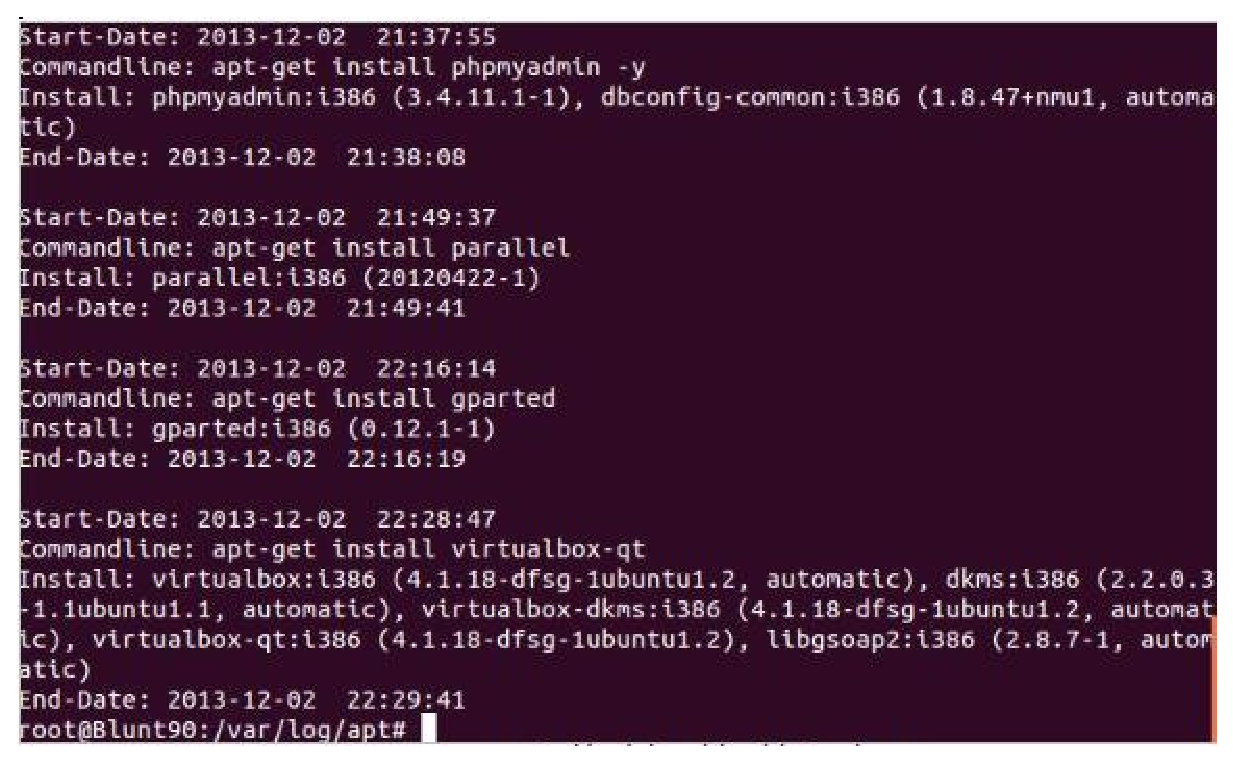
\includegraphics[scale=0.6]{imagenes/ejercicio1.eps}
\caption{Resultado de la operación "cat /var/log/apt/history.log".}
\end{center}
\end{figure}

\footnote{http://unix.stackexchange.com/questions/12578/list-packages-by-installation-date}

\subsection{¿Qué significan las terminaciones .1.gz o .2.gz de los archivos en ese directorio?}
Según tengo entendido son archivos de registro comprimidos.

Indican antigüedad, siendo ".1.gz" la más reciente y ".i.gz" con i>1 posterior a 1.
Y por supuesto "gz" quiere decir que está comprimido en "gzip".

\section{¿qué archivo ha de modificar para programar una tarea? Escriba la línea necesaria para ejecutar una vez al día una copia del directorio ~/codigo a ~/seguridad/$fecha donde $fecha es la fecha actual (puede usar el comando date).}

Hay que introducir la fecha y la hora en la que queremos ejecutar el script e indicarlo con el formato que entiende "cron".
Normalmente "cron" esta activo, pero si no es asi, podemos activarlo con : service cron start.

Para realizar esta practica se crea un script, en el que estara programada la tarea de comprimir el directorio codigo y se copiara en la carpeta segura dentro de una subcarpeta cuyo nombre sera el dia en que se realiza esta copia.

\begin{figure}[H]
\begin{center}
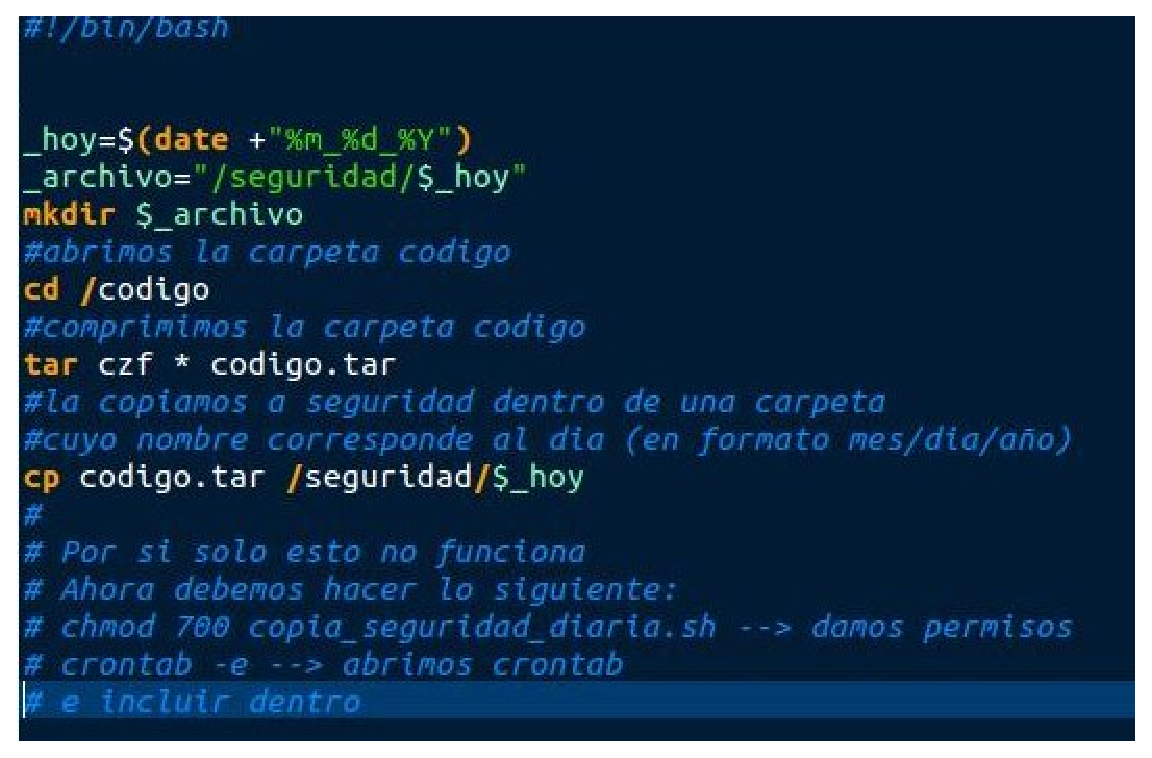
\includegraphics[scale=0.6]{imagenes/ejercicio2.eps}
\caption{Script creado para programar la tarea indicada.}
\end{center}
\end{figure}


Una vez hecho el script, para que este funcione deberemos modificar el archivo /etc/crontab".

Podemos hacer esto desde terminal ejecutando crontab -e , e introduciendo una linea, donde debemos indicar el momento exacto en el que se deberá ejecutarse, puesto que queremos que sea todos los días pondremos que se haga todos los dias a las 5 de la mañana, también debemos indicar el archivo que se ejecutará, con lo que nos quedará algo asi:


00 5 * * * root /usr/script\_cron.sh 
\linebreak

Introduciendo la linea anterior en crontab harémos que el archivo script\_cron.sh se ejecute todos los días a las 5 de la mañana.

\footnote{https://docs.oracle.com/cd/E26921\_01/html/E25809/sysrescron-1.html}

\section{Pruebe a ejecutar el comando, conectar un dispositivo USB y vuelva a ejecutar el comando. Copie y pegue la salida del comando. (considere usar dmesg | tail). Comente qué observa en la información mostrada.}

En primer lugar ejecutamos el comando sin el USB conectado, lo que nos muestra el siguiente resultado:

\begin{figure}[H]
\begin{center}
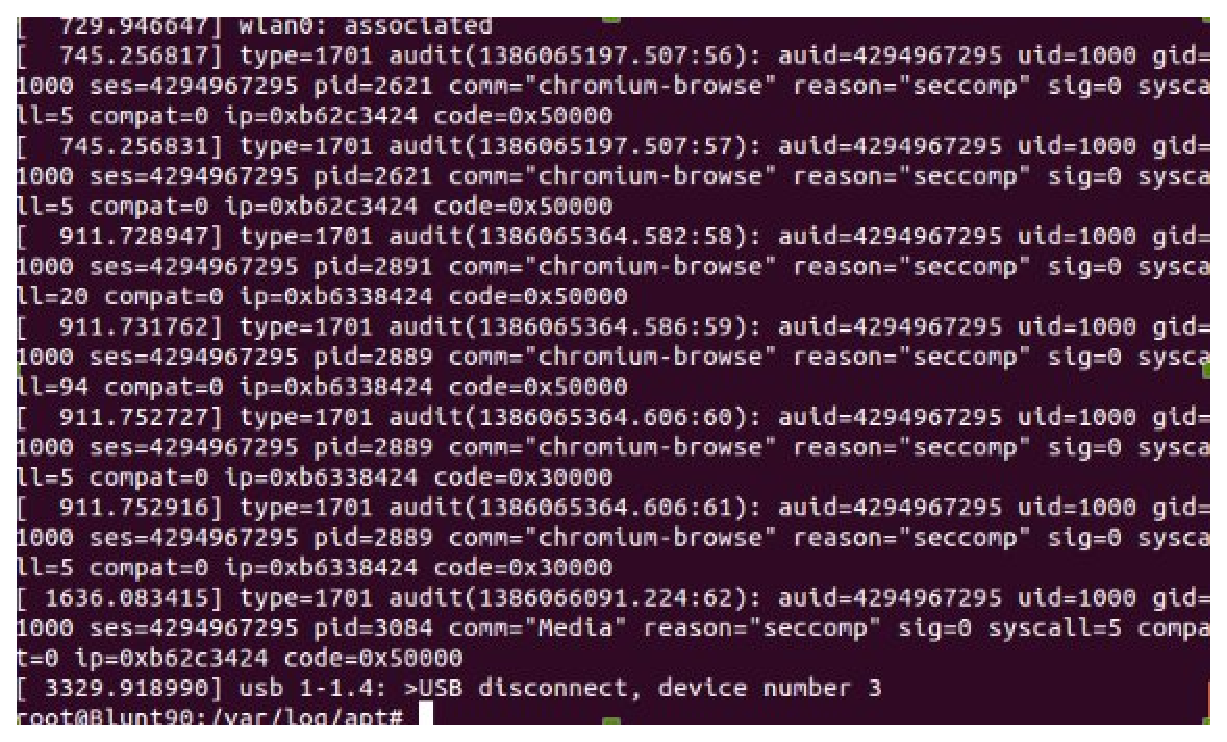
\includegraphics[scale=0.6]{imagenes/ejercicio3-1.eps}
\caption{Ejemplo sin el USB conectado.}
\end{center}
\end{figure}

Ahora volvemos a ejecutarlo con el USB conectado, el resultado es el siguiente:


\begin{figure}[H]
\begin{center}
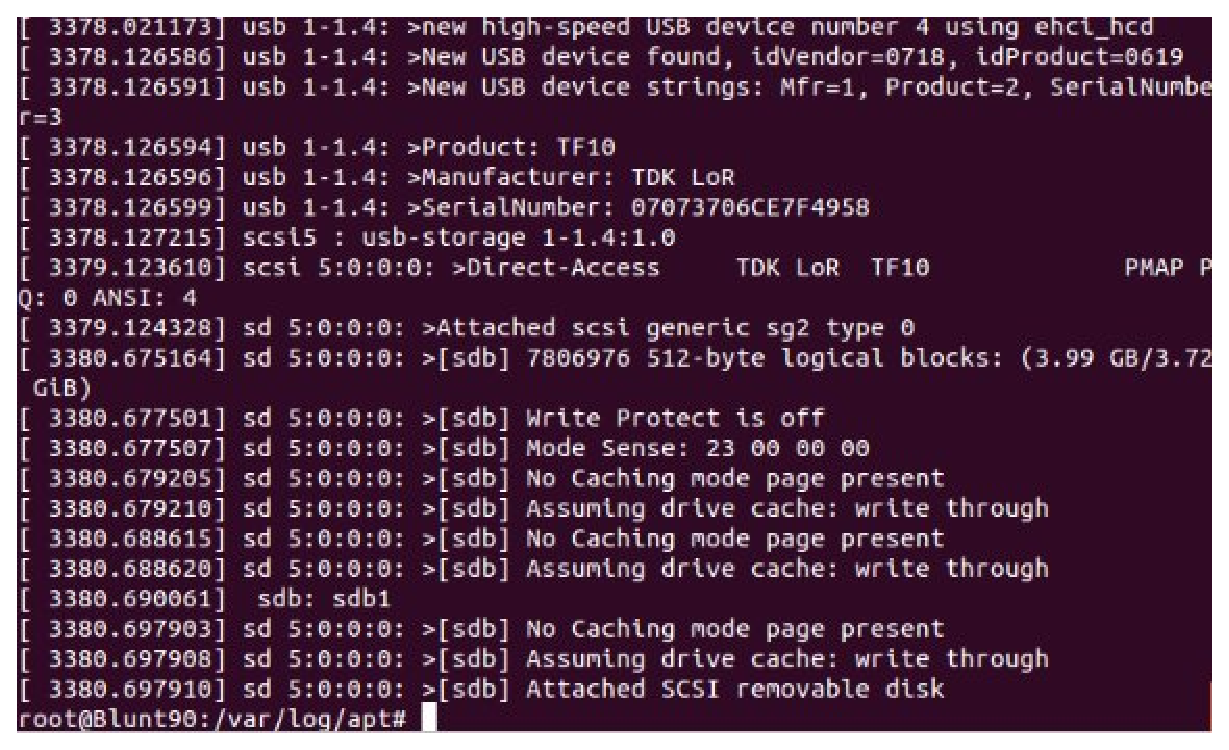
\includegraphics[scale=0.6]{imagenes/ejercicio3-2.eps}
\caption{Ejemplo con el USB conectado.}
\end{center}
\end{figure}

Una vez redireccinemos a tail el comando nos presentara como resultado los últimos acontecimientos producidos en el sistema.

\begin{figure}[H]
\begin{center}
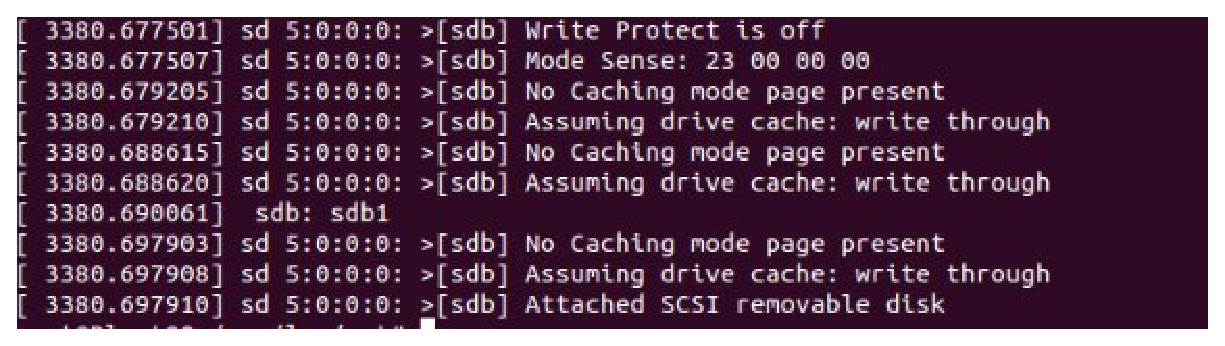
\includegraphics[scale=0.6]{imagenes/ejercicio3-3.eps}
\caption{Ejemplo con el uso de tail.}
\end{center}
\end{figure}

\footnote{http://debianfacil.wordpress.com/2013/04/15/dmesg/}

\section{ Ejecute el monitor de “System Performance” y muestre el resultado. Incluya capturas de pantalla comentando la información que aparece.}

Ponemos "perfmon" en la lista de comandos y nos saldrá la ventana siguiente:

\begin{figure}[H]
\begin{center}
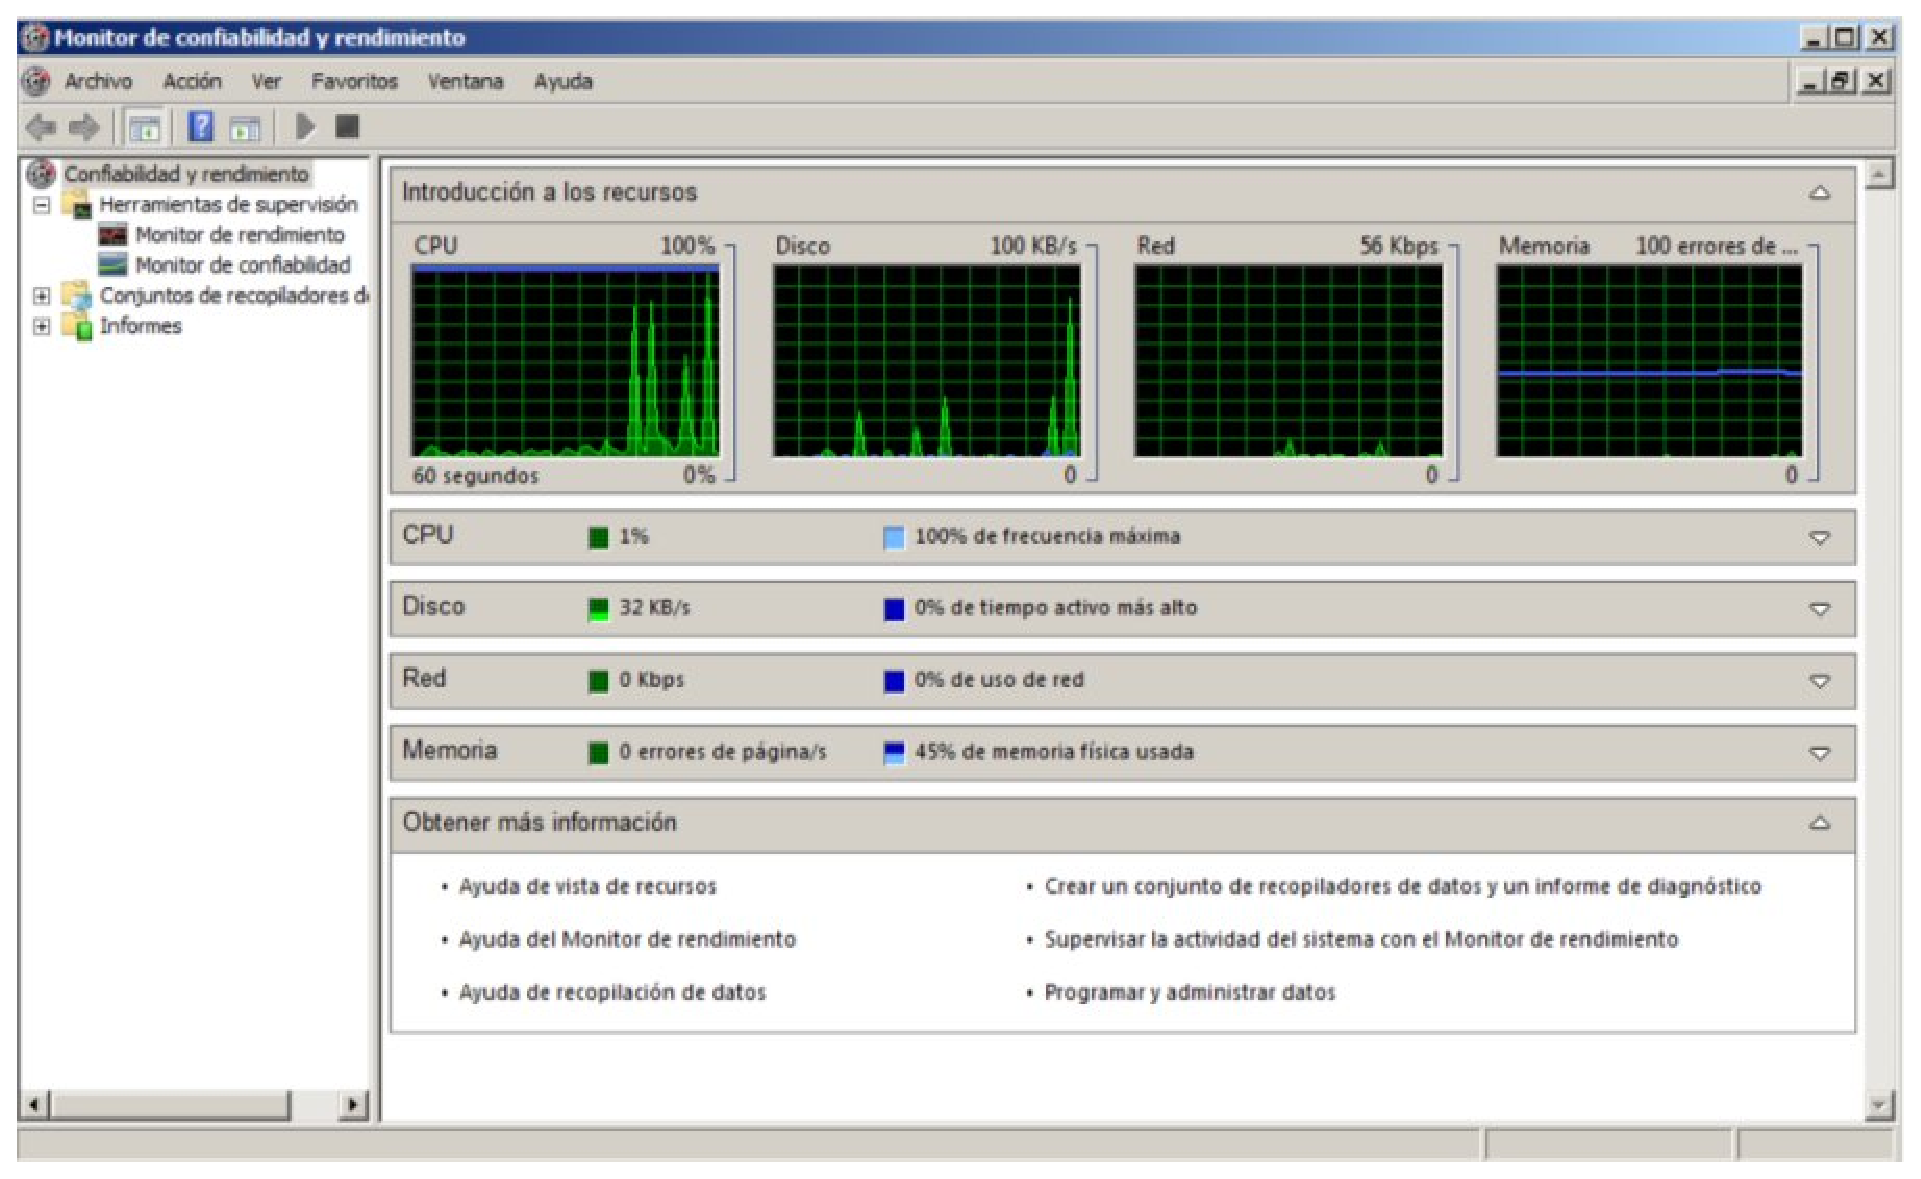
\includegraphics[scale=0.4]{imagenes/ejercicio4-1.eps}
\caption{Ventana principal de " System Performance".}
\end{center}
\end{figure}

Por ejemplo, podemos ver la memoria que está siendo utilizada y por quién.

Desplegamos la pestaña de "Memoria":


\begin{figure}[H]
\begin{center}
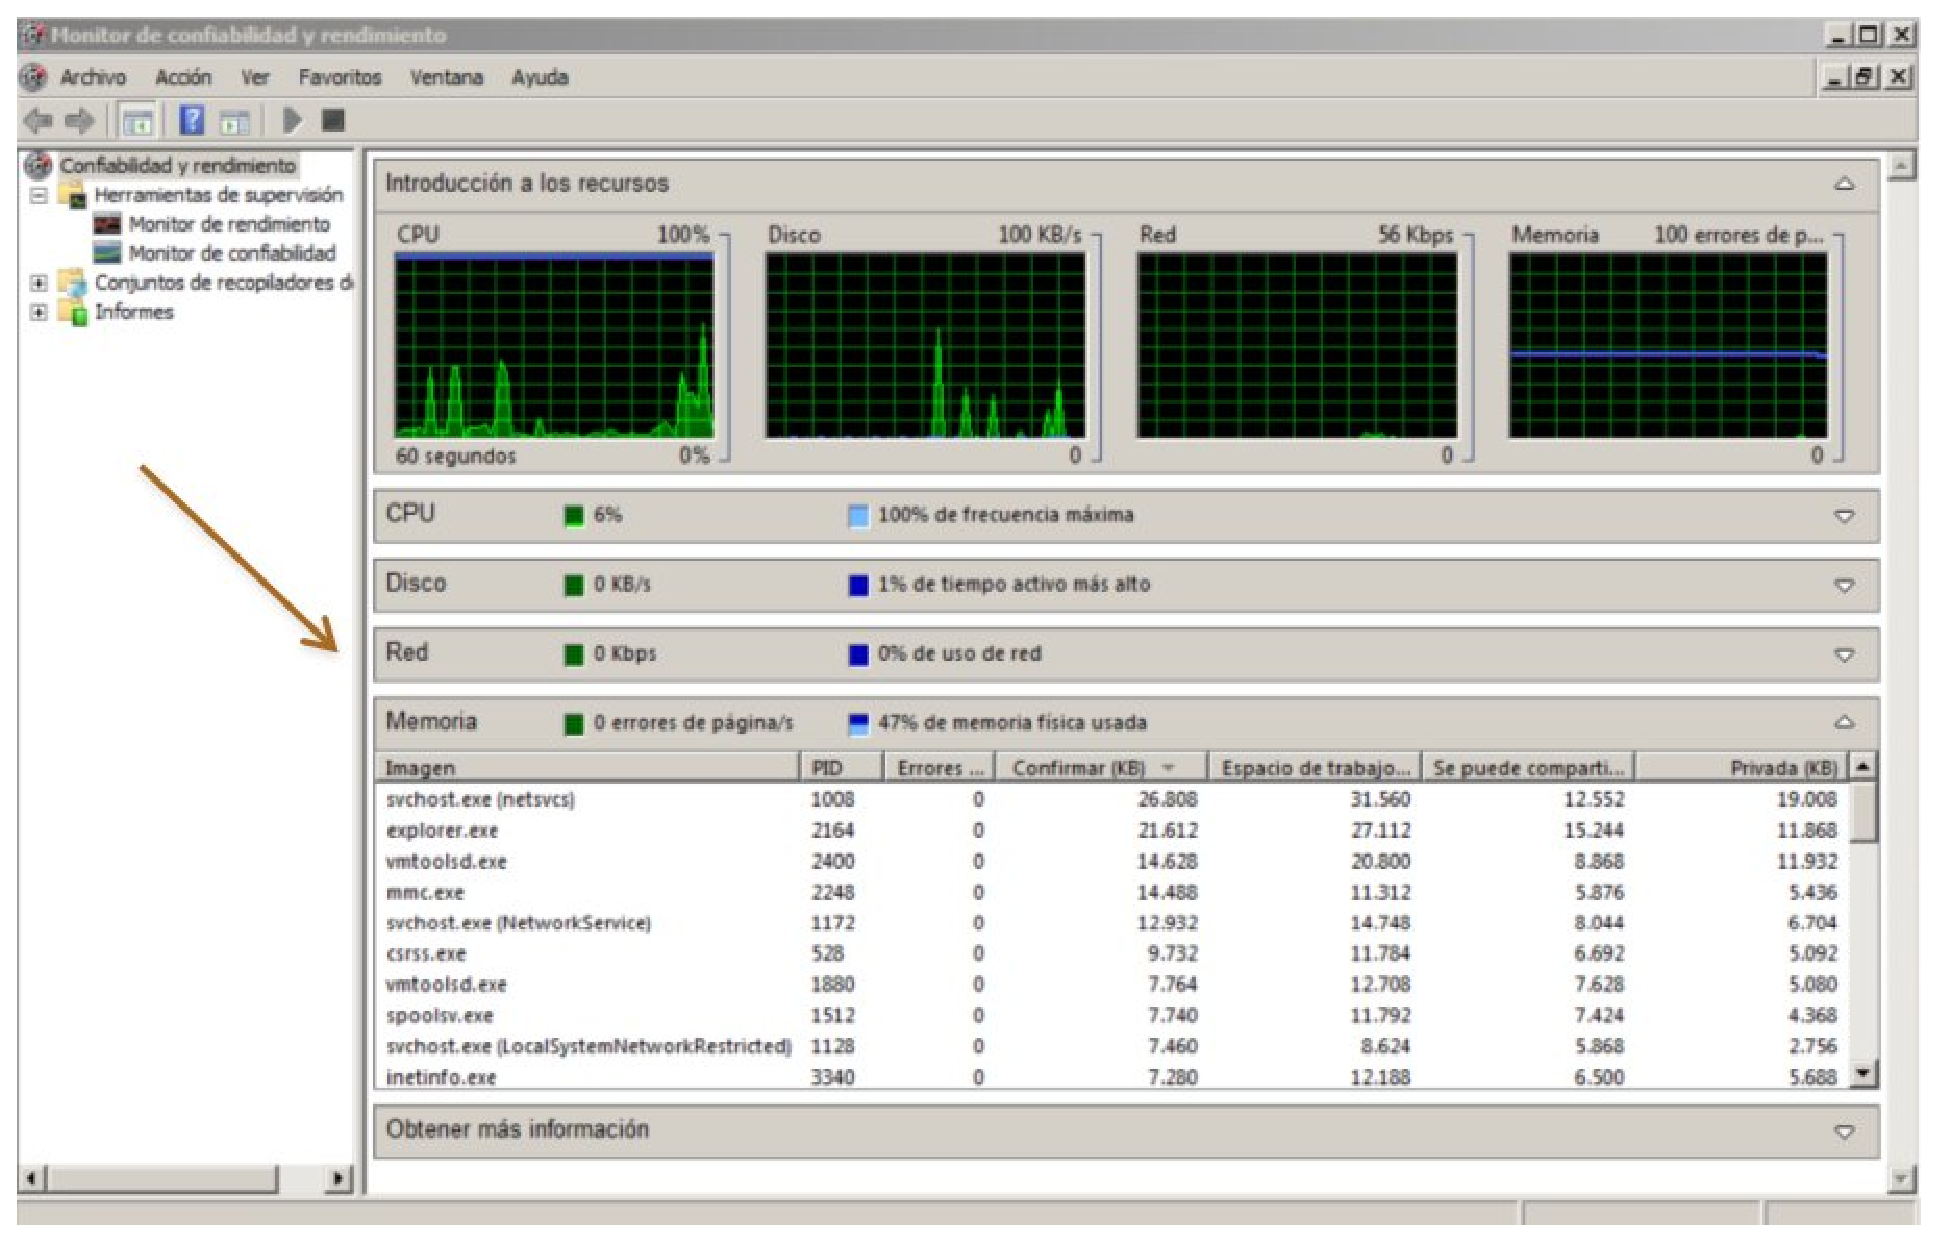
\includegraphics[scale=0.4]{imagenes/ejercicio4-2.eps}
\caption{Pestaña de Memoria en System Performance.}
\end{center}
\end{figure}

Entre otras opciones también podriamos ver el rendimiento del sistema haciendo click en su mismo nombre:

\begin{figure}[H]
\begin{center}
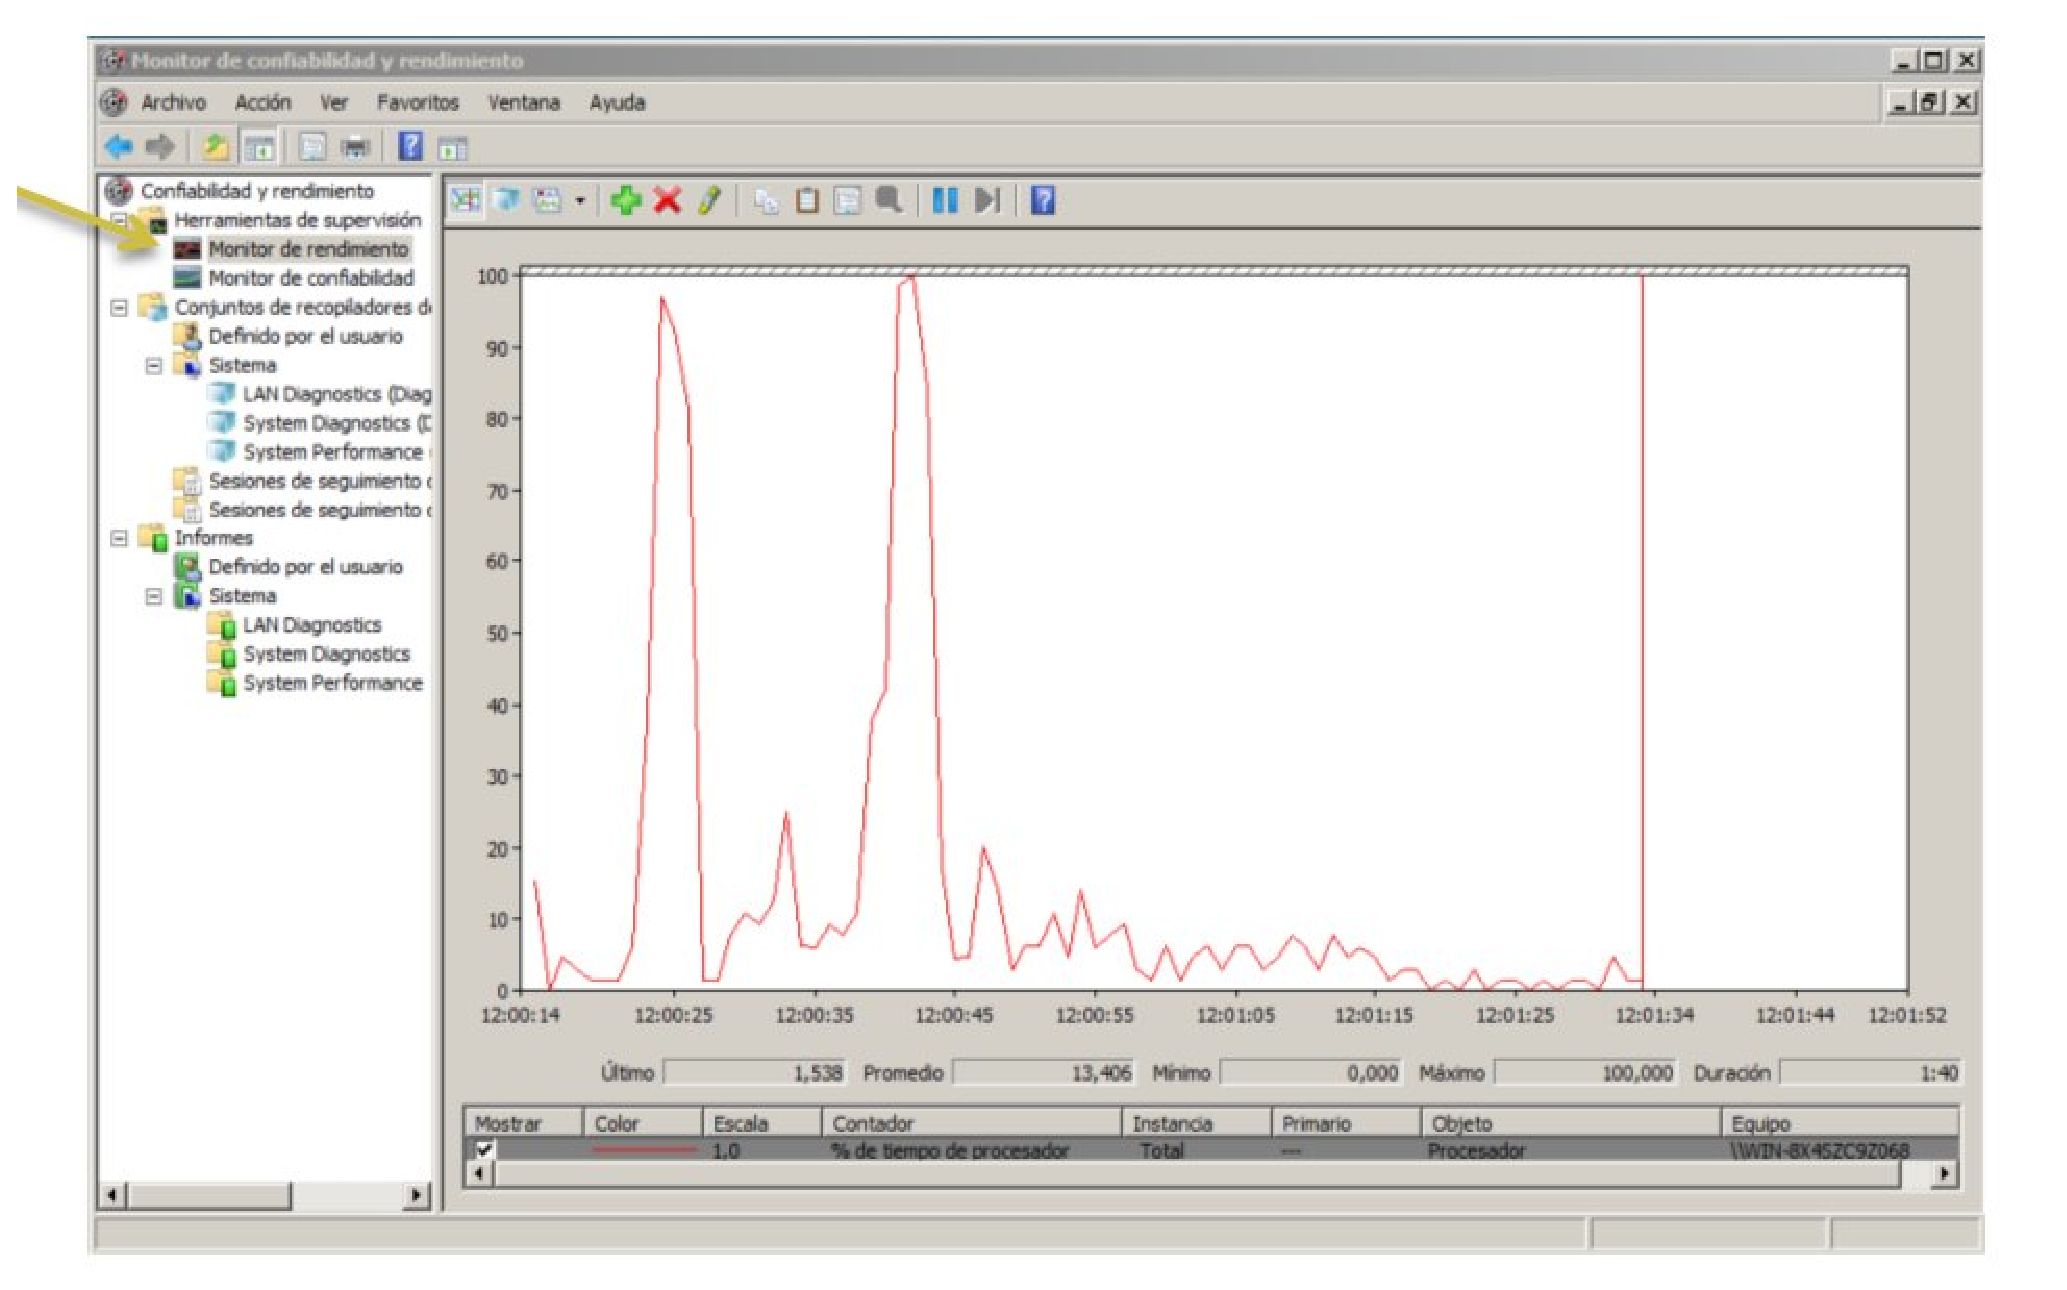
\includegraphics[scale=0.4]{imagenes/ejercicio4-3.eps}
\caption{Rendimiento del sistema.}
\end{center}
\end{figure}

Este comando muestra, en los 1:40 minutos que llevamos de tiempo, el rendimiento que al principio ha ido al máximo (algo extraño, puesto que se supone que no habia nada ejecutandose mas que esto).

\footnote{http://technet.microsoft.com/en-us/library/cc749154.aspx}

\section{ Cree un recopilador de datos definido por el usuario (modo avanzado) que incluya tanto el contador de rendimiento como los datos de seguimiento: Todos los referentes al procesador, al proceso y al servicio web. Intervalo de muestra 15 segundos. Almacene el resultado en el directorio Escritorio\textbackslash{}logs Incluya las capturas de pantalla de cada paso.}

Para esto lo que tenemos que hacer es irnos a definir un nuevo Conjunto de recopilador de datos.

Como se muestra en la siguiente figura.

\begin{figure}[H]
\begin{center}
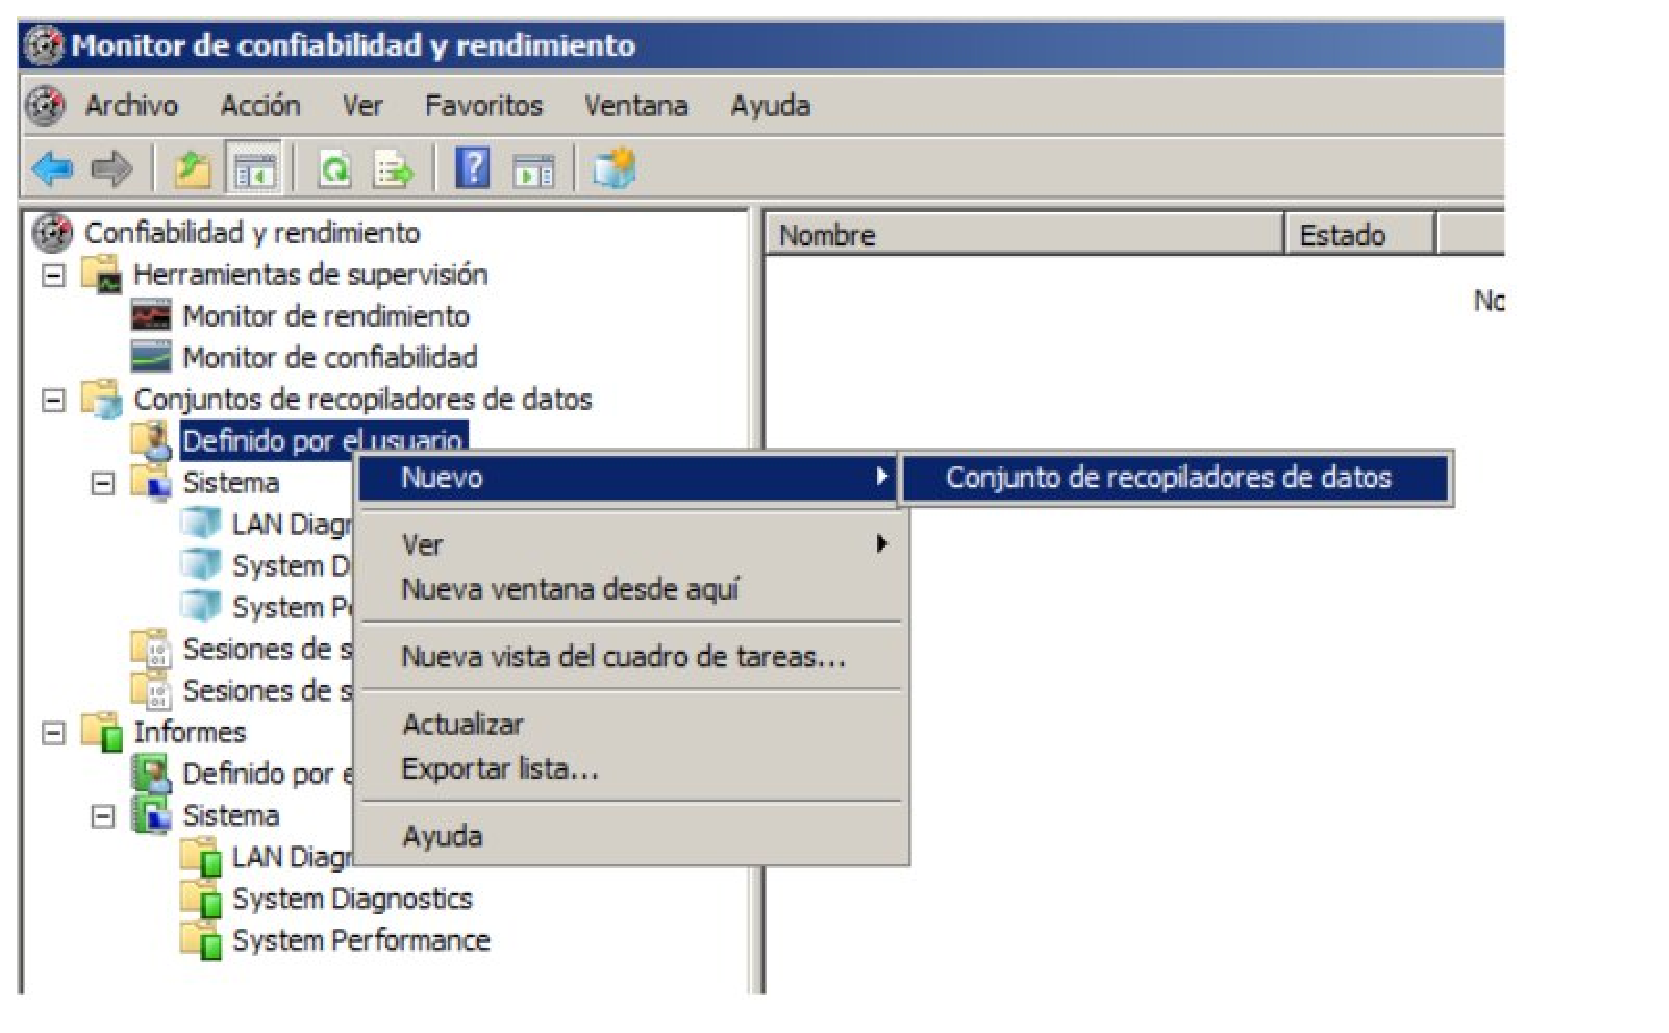
\includegraphics[scale=0.4]{imagenes/ejercicio5-1.eps}
\caption{Crear recopilador de datos.}
\end{center}
\end{figure}

Nos aparecera una venta en la que unicamente deberemos introducir el nombre del recopilador y seleccionamos la opción de "crear manualmente (avanzado)".

Ahora debemos seleccionar el tipo de datos que deseamos incluir en nuestro recopilador.



\begin{figure}[H]
\begin{center}
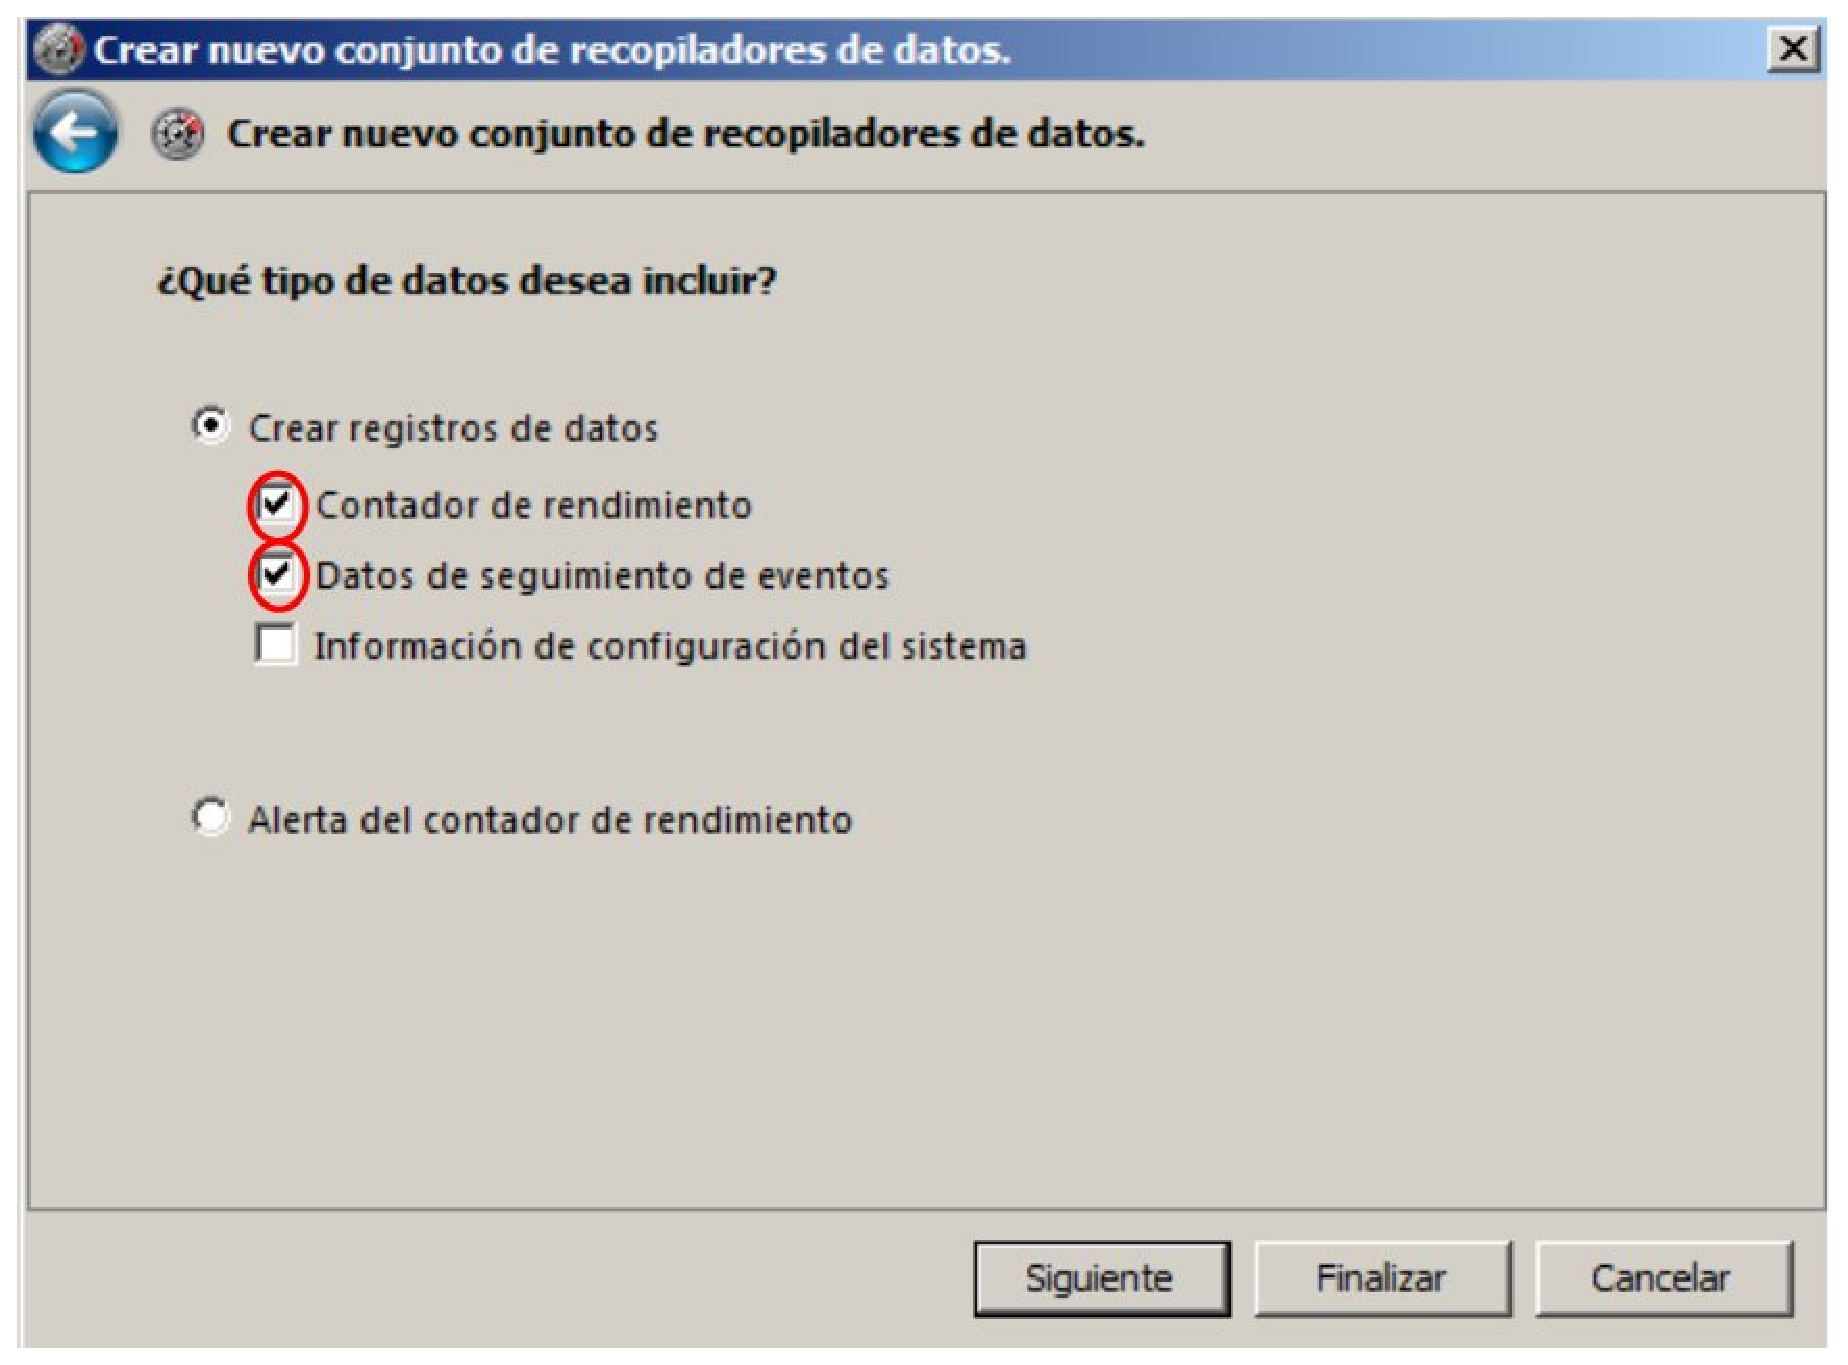
\includegraphics[scale=0.4]{imagenes/ejercicio5-3.eps}
\caption{Seleccion de tipos de datos para el recopilador.}
\end{center}
\end{figure}

En este punto  seleccionamos los contadores, escojemos contadores para el procesador, procesos y todo lo relacionado con servicio web.

\begin{figure}[H]
\begin{center}
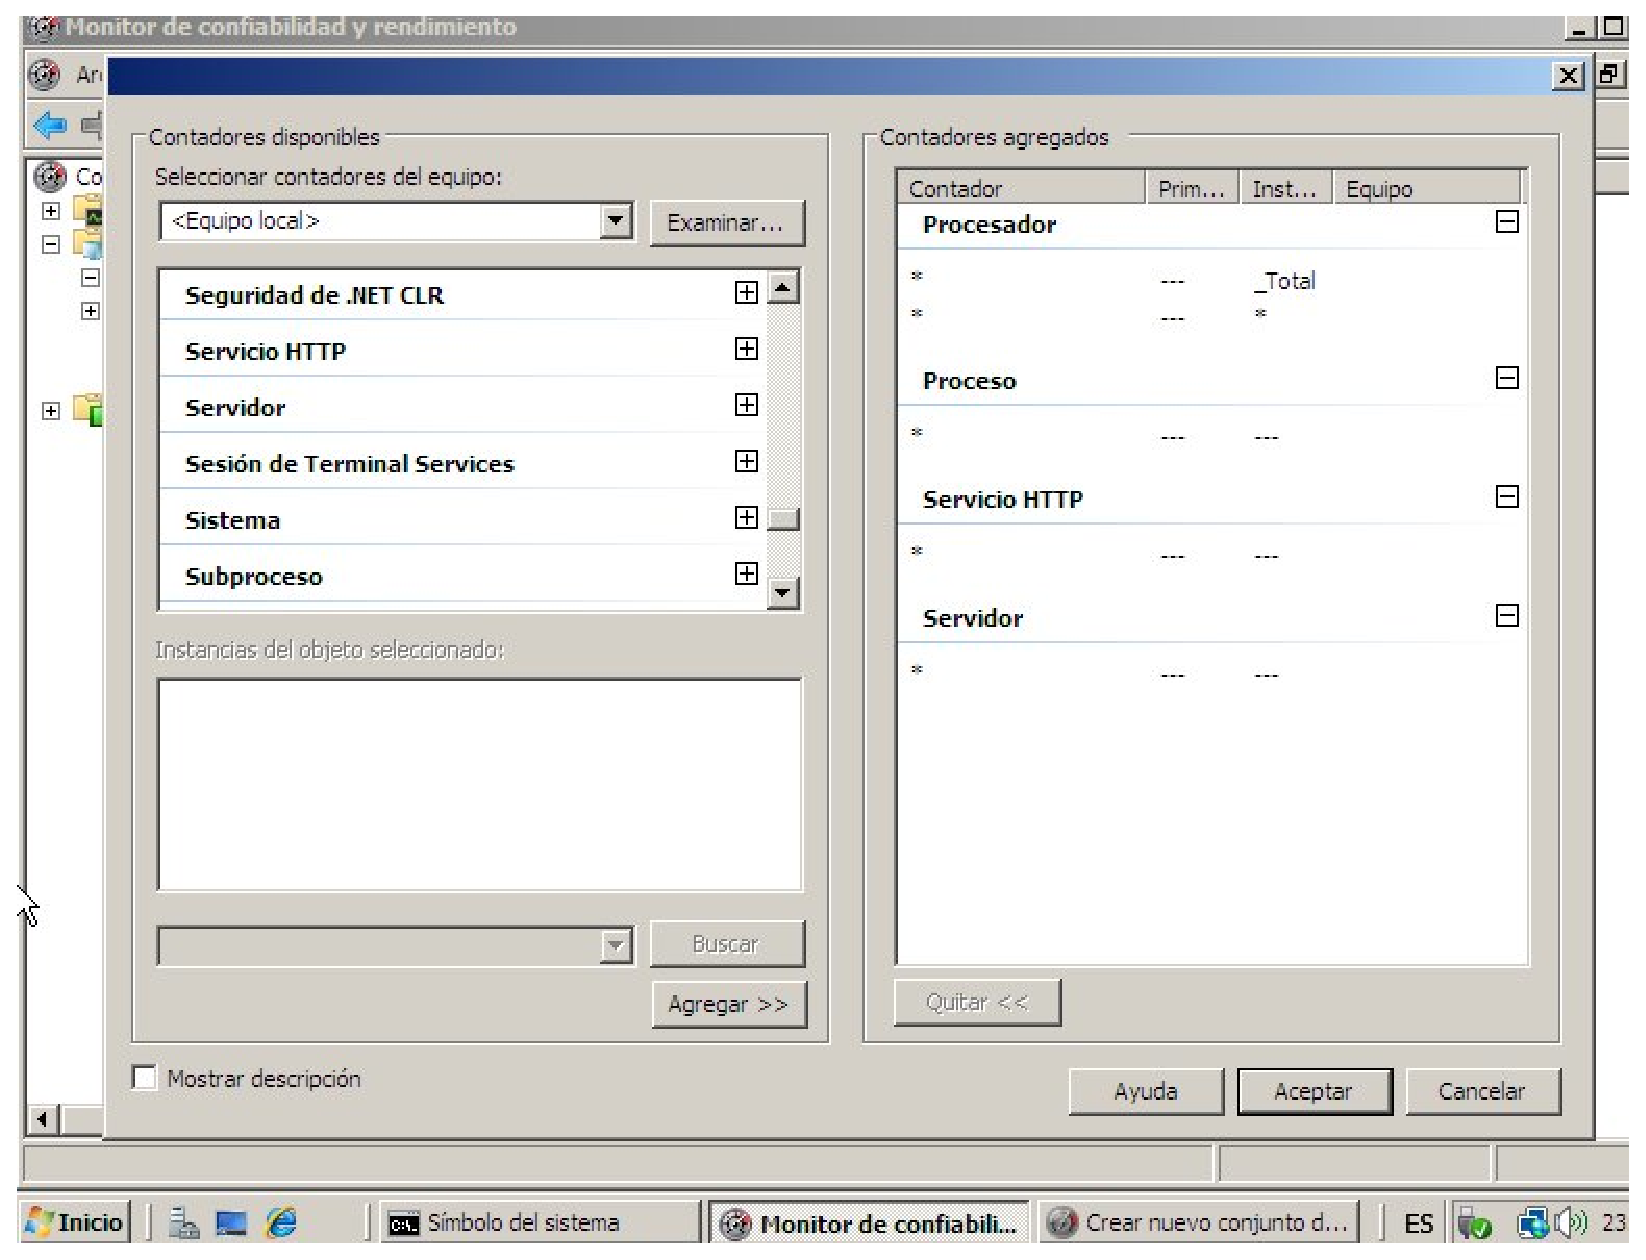
\includegraphics[scale=0.4]{imagenes/ejercicio5-4.eps}
\caption{Seleccion de contadores para el recopilador.}
\end{center}
\end{figure}

Y ya lo tenemos todo listo.

En caso de que nuestro recopilador no este activo pinchamos sobre el y lo activamos. 

\begin{figure}[H]
\begin{center}
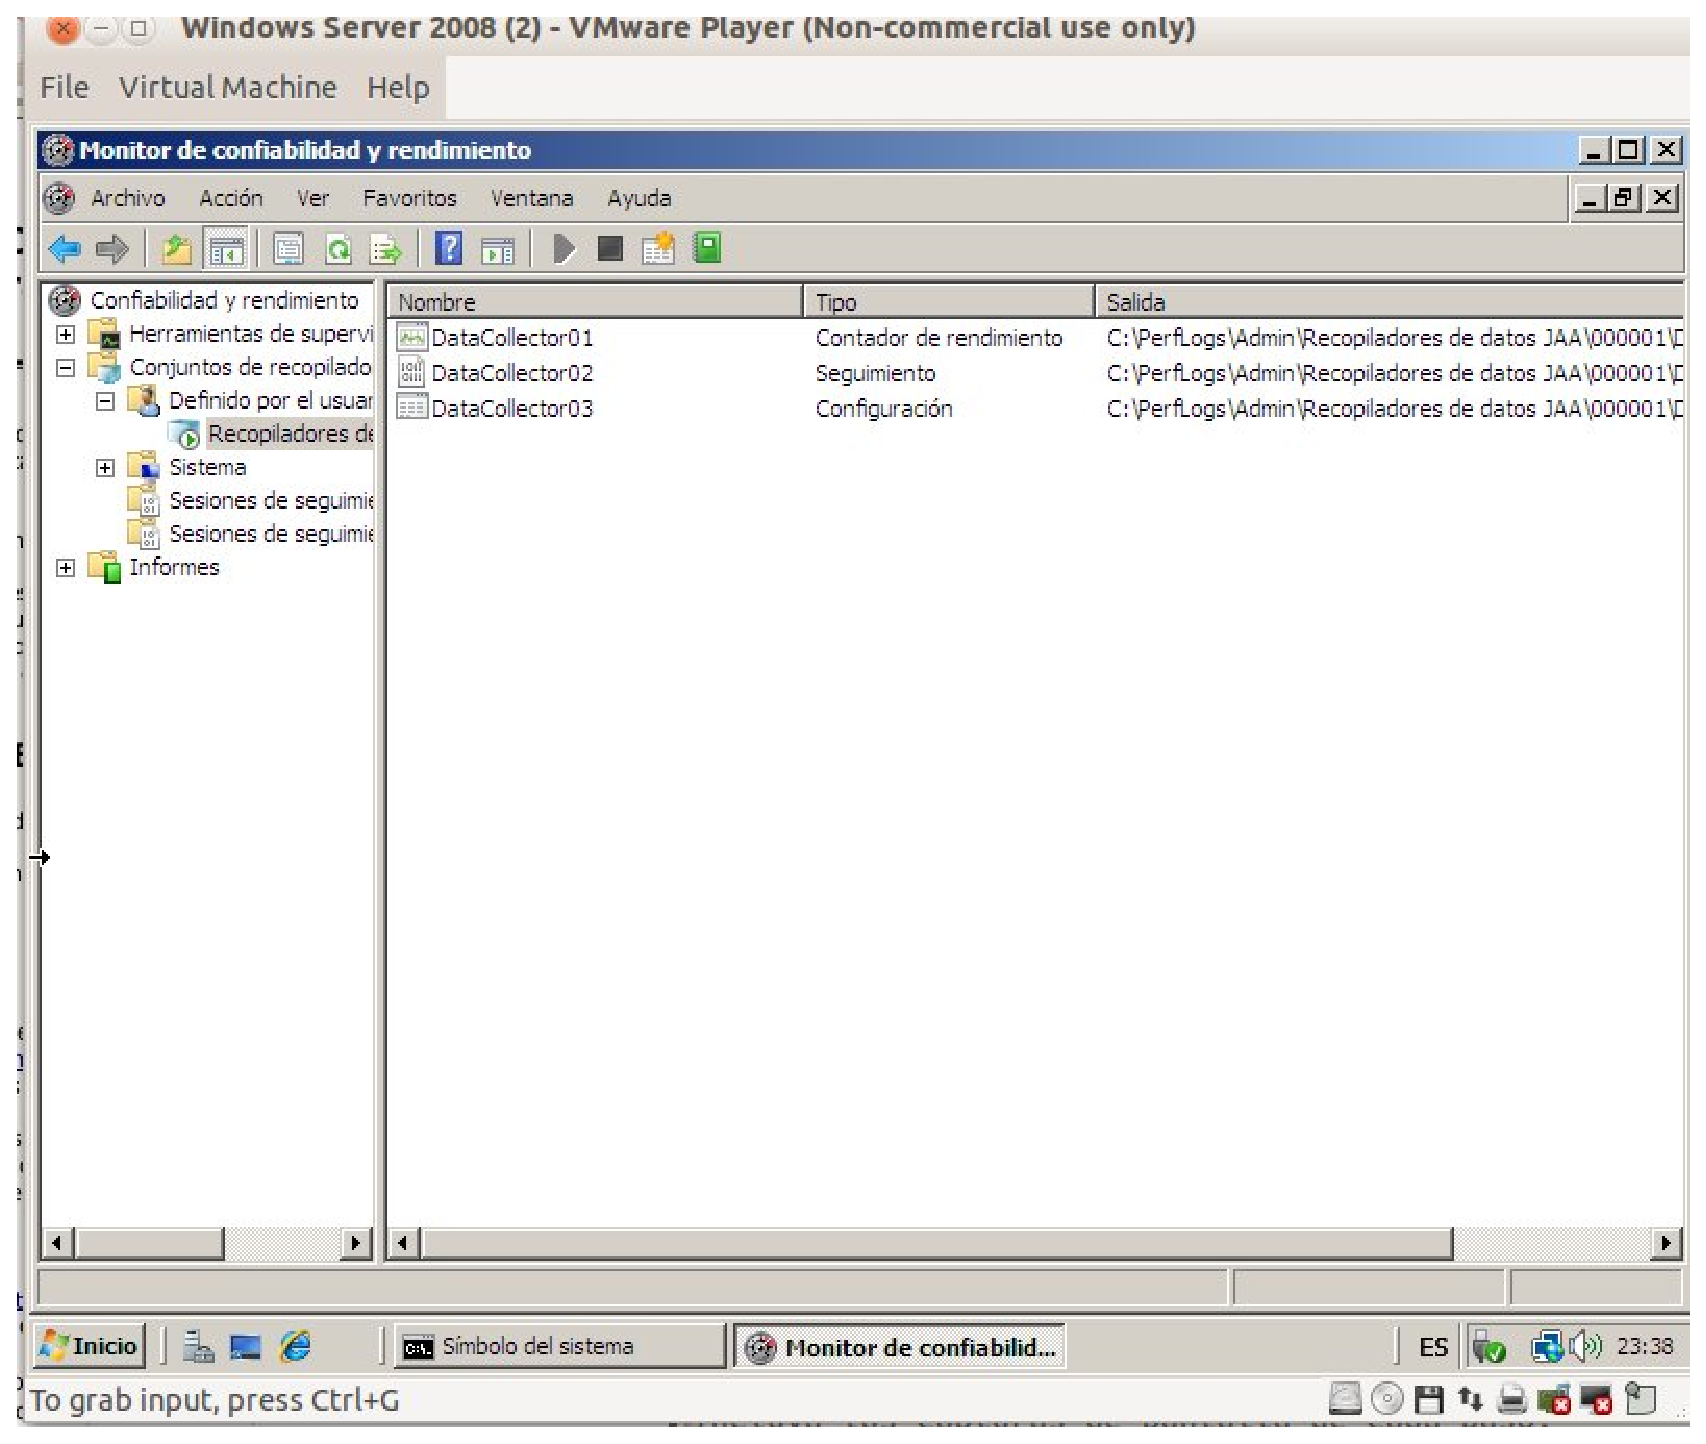
\includegraphics[scale=0.4]{imagenes/ejercicio5-5.eps}
\caption{Imagen del contador de rendimiento listo para iniciarse.}
\end{center}
\end{figure}


\section{Instale alguno de los monitores comentados arriba en su máquina y pruebe a ejecutarlos (tenga en cuenta que si lo hace en la máquina virtual, los resultados pueden no ser realistas). Alternativamente, busque otros monitores para hardware comerciales o de código abierto para Windows y Linux. }

He instalados hddtemp junto a lm-sensors en Ubuntu. El uso de hddtemp es para poder ver la temperatura del disco. Este programa permite controlar la temperatura del hardware en el que esta instalado el sistema.



Para descargar e instalar lm-sensor meti el archivo en los repositorios y posteriormente los descomprimí.
\\
wget http://dl.lm-sensors.org/lm-sensors/rel ... .0.tar.bz2
\\
bzip2 -dv lm\_sensors-3.2.0.tar.bz2
\\
tar xvf lm\_sensors-3.2.0.tar

Después pasamos a ejecutar:

yum install lm\_sensors


\begin{figure}[H]
\begin{center}
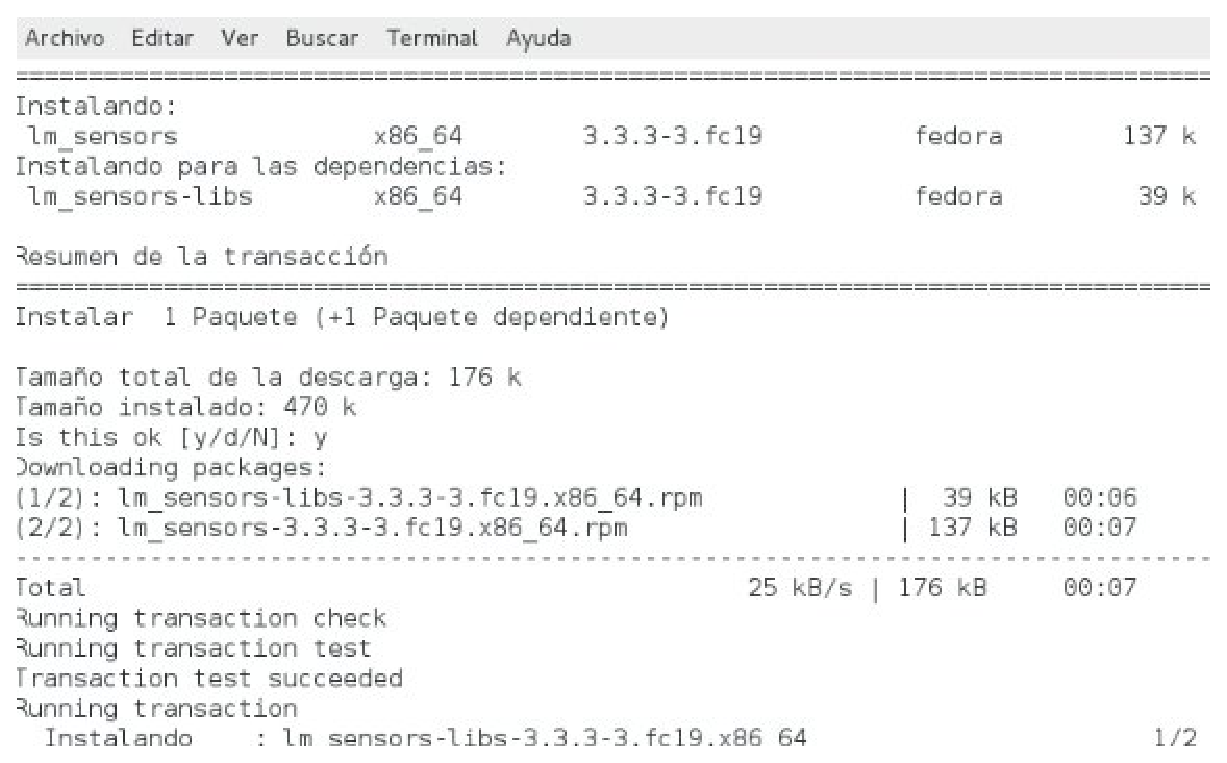
\includegraphics[scale=0.6]{imagenes/ejercicio6-1.eps}
\caption{Instalación lm-sensors.}
\end{center}
\end{figure}

 wget http://download.savannah.gnu.org/releases/hddtemp/hddtemp-0.3-beta15.tar.bz2

tar -jxvf hddtemp-0.3-beta15.tar.bz2

Nos introducimos en la carpeta "hddtemp-0.2-beta15"
 Y hacemos "make" y "make install"

\begin{figure}[H]
\begin{center}
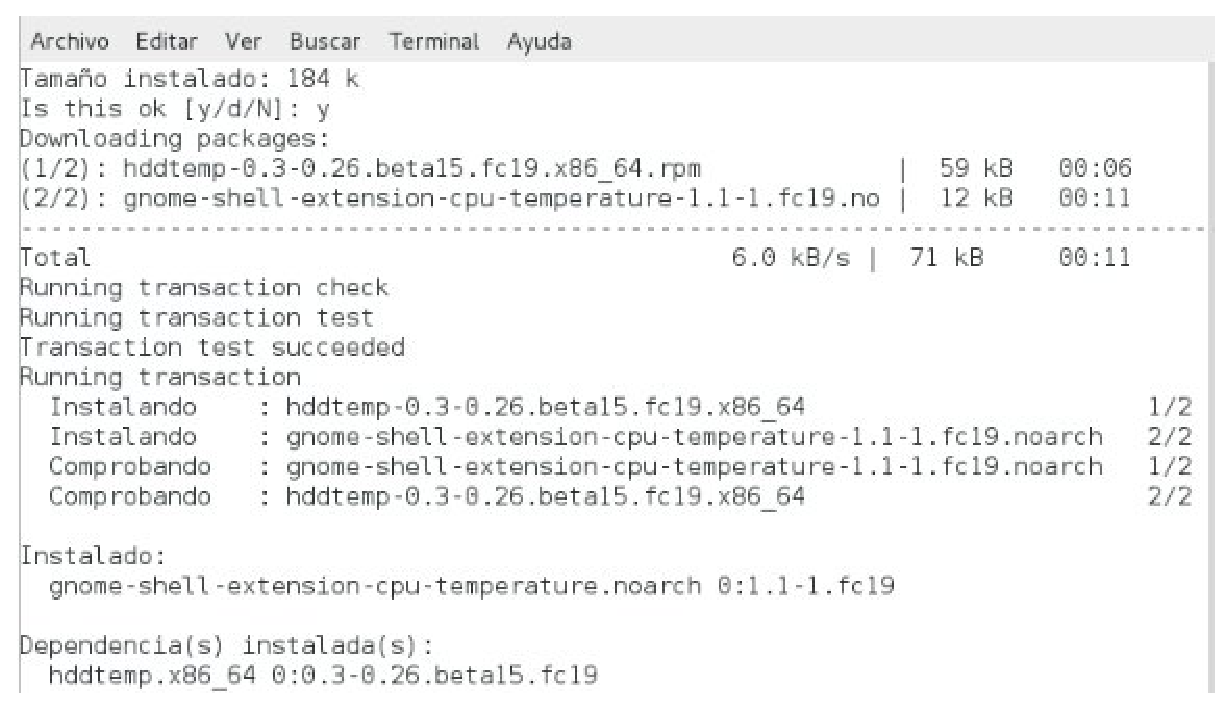
\includegraphics[scale=0.6]{imagenes/ejercicio6-5.eps}
\caption{Instalación hddtemp.}
\end{center}
\end{figure}



Una vez instalado ejecutamos :

sensors-detect.

\begin{figure}[H]
\begin{center}
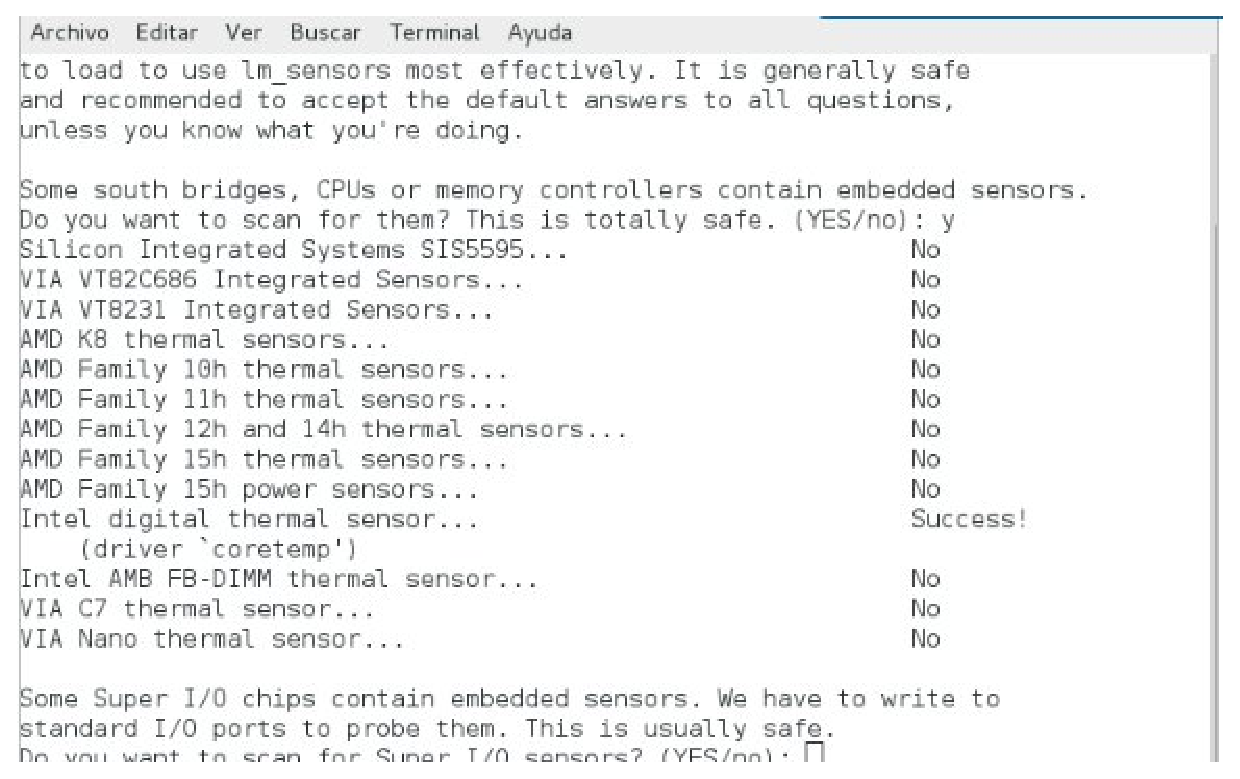
\includegraphics[scale=0.6]{imagenes/ejercicio6-6.eps}
\caption{Ejecucion sensors-detect.}
\end{center}
\end{figure}

Este comando nos sirve para ver que dispositivos se pueden monitorear. Ahora para comprobar el estado podemos ejecutar : sensors, y asi comprobar el estado.

\footnote{http://technet.microsoft.com/en-us/library/cc749154.aspx}
\footnote{https://wiki.archlinux.org/index.php/Hddtemp}

\section{ Visite la web del proyecto y acceda a la demo que proporcionan (http://demo.munin-monitoring.org/) donde se muestra cómo monitorizan un servidor. Monitorice varios parámetros y haga capturas de pantalla de lo que está mostrando comentando qué observa.}

Munin permite recopilar informacion muy diversa sobre el sistema.

Por ejemplo entre otras cosas permite controlar los accesos a internet y las visitas a paginas que hacer los usuarios del sistema.

Tiene muchas opciones como son el control de los procesos, monitorización de los repositorios de Github,etc.

Dentro del enlace proporcionado nos aparecerá la siguiente ventana. 

\begin{figure}[H]
\begin{center}
\includegraphics[scale=0.3]{imagenes/Munin1.eps}
\caption{Pagina principal de la demos de Munin.}
\end{center}
\end{figure}

Pinchamos en " munin-monitoring.org" o en "demo.munin-monitorin.org".

Si pinchamos en la primera opción nos saldra las siguiente imagen.

\begin{figure}[H]
\begin{center}
\includegraphics[scale=0.3]{imagenes/Munin2.eps}
\caption{Eleccion de parámetros a monitorizar dentro de la demo.}
\end{center}
\end{figure}

Pinchamos por ejemplo en la opción "Number of threads".

\begin{figure}[H]
\begin{center}
\includegraphics[scale=0.3]{imagenes/Munin3.eps}
\caption{Conjunto de gráficas de ejemplo relacionada con los procesos.}
\end{center}
\end{figure}

Y en la opción "Number of threads By year"

\begin{figure}[H]
\begin{center}
\includegraphics[scale=0.2]{imagenes/Munin4.eps}
\caption{Diferentes graficos sobre el numero de hebras segun un periodo de tiempo.}
\end{center}
\end{figure}

Aquí se nos permite seleccionar algunos parámetros.

Podemos seleccionar con un par de clicks un periodo de tiempo y volviendo a pinchar sobre el se ajustará a los parámetros seleccionados además del periodo de tiempo seleccionado.

\begin{figure}[H]
\begin{center}
\includegraphics[scale=0.2]{imagenes/Munin5.eps}
\caption{Seleccion de un periodo de tiempo.}
\end{center}
\end{figure}

Si retocamos los parámetros podemos  ver con mas claridad los resultados de monitoreo.


\begin{figure}[H]
\begin{center}
\includegraphics[scale=0.2]{imagenes/Munin6.eps}
\caption{Ajuste del periodo según lo indicado anteriormente.}
\end{center}
\end{figure}



\section{Escriba un breve resumen sobre alguno de los artículos donde se muestra el uso de strace o busque otro y coméntelo.}


Para el resumen he usado el segundo enlace: \url{ http://blog.softlayer.com/2013/sysadmin-tips-and-tricks-using-strace-to-monitor-system-calls#utm_source=twitter&utm_medium=social&utm_content=beyond-the-command-line-with-strace&utm_campaign=blog_development-tips-and-tricks}.

El articulo comienza explicando que es y que no es "strace". Es una herramienta para administradores de sistemas con la que es "posible mantener un seguimiento de las llamadas al sistema y señales".

Lo único que se necesita es conectar a strace con el proceso para que nos muestre las llamadas al sistema y las señales que resultan de ese proceso, aunque lo verdaderamente importante es que strace devuelve informacion sobre los resultados del comando junto a los errores que encontró.

El articulo muestra un par de ejemplos bastante explicativos sobre el funcionamiento de strace.




\section{Acceda a la consola mysql (o a través de phpMyAdmin) y muestre el resultado de mostrar el ”profile” de una consulta (la creación dela BD y la consulta la puede hacer líbremente).}

En la primera imagen se ve el resultado de una consulta y el profile de esta.

\begin{figure}[H]
\begin{center}
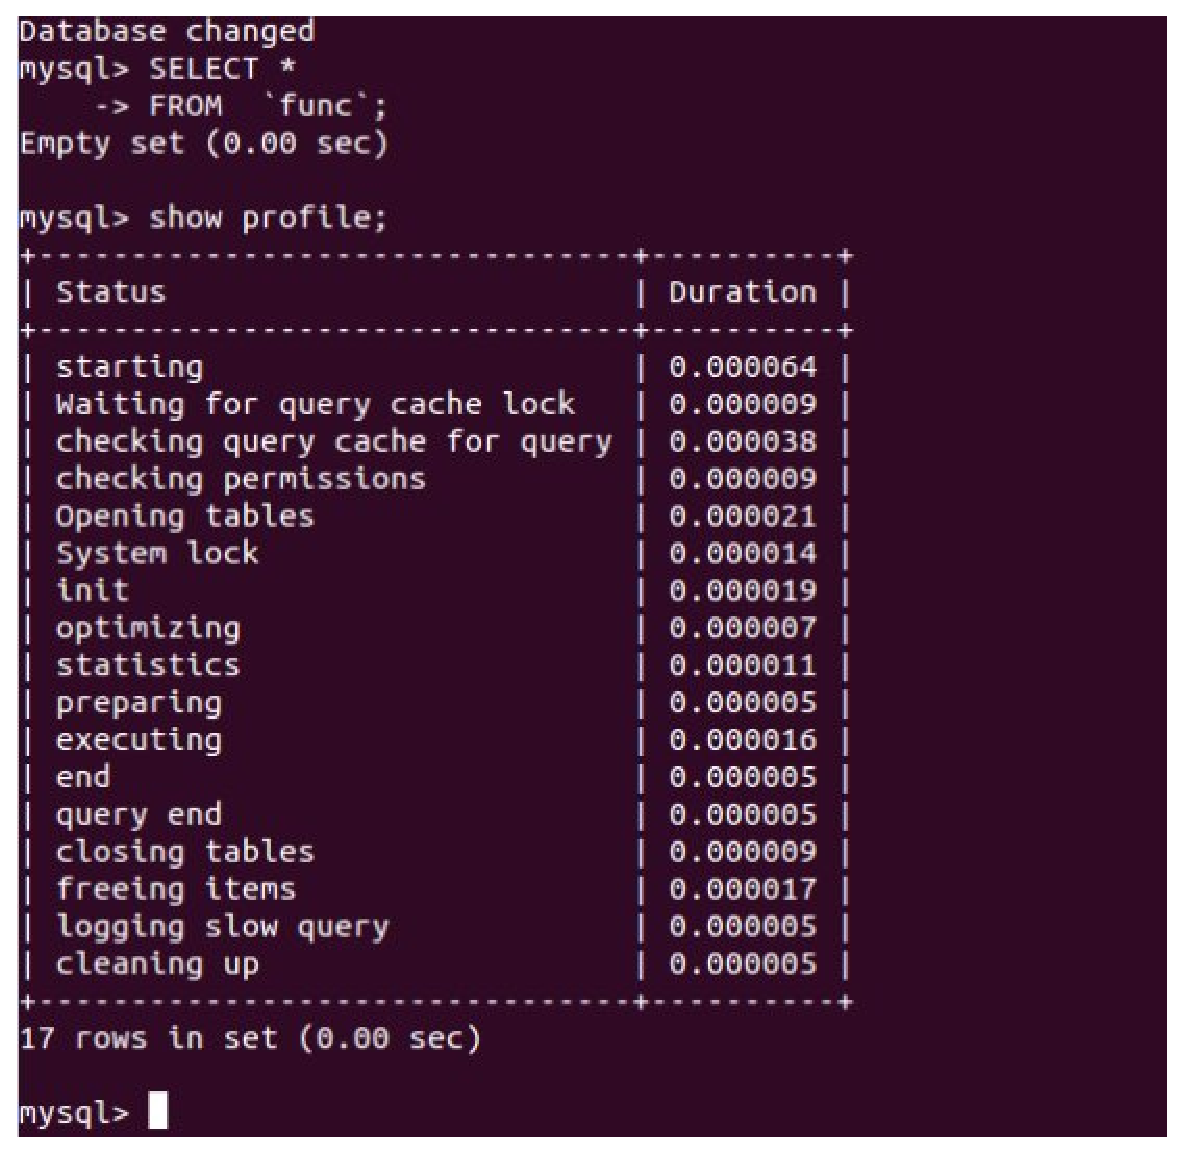
\includegraphics[scale=0.4]{imagenes/ejercicio9-1.eps}
\caption{Ejecución de profile en SQL.}
\end{center}
\end{figure}

La siguiente imagen muestra el tiempo de ejecución de phpMyadmin de la misma consulta.

\begin{figure}[H]
\begin{center}
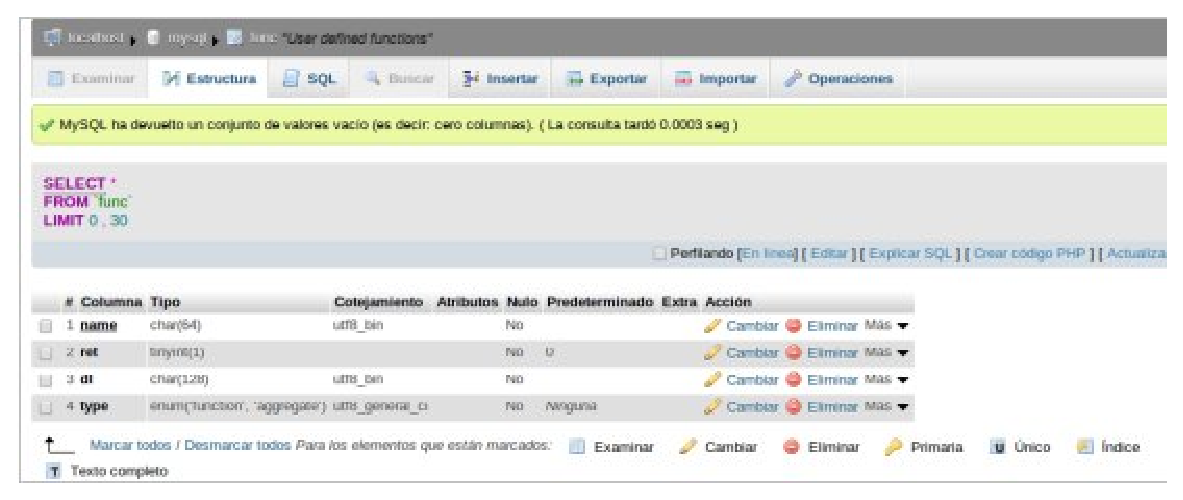
\includegraphics[scale=0.4]{imagenes/ejercicio9-2.eps}
\caption{Resultado de consulta en phpMyAdmin.}
\end{center}
\end{figure}

\footnote{Para esta cuestión me ayudó el profesor el año pasado.}

%----------------------------------------------------------------------------------------
%--- OPCIONALES--------------------
%----------------------------------------------------------------------------------------
%----------------------------------------------------------------------------------------

\section*{Cuestion opcional 2 : Instale Nagios en su sistema (el que prefiera) documentando el proceso y muestre el resultado de la monitorización de su sistema comentando qué aparece}

Todos los pasos los realizaremos como root. Para la realización de esta instalación me he ayudado de un tutorial que he encontrado buscando en google.\footnote{drivemeca.blogspot.com.es/2013/04/como-instalar-nagios-en-centos-64-
paso.html}

Creamos el usuario “nagios” y le asignamos una contraseña. Además crearemos el
grupo de ejecución de comandos que usará la interfaz web:

\begin{itemize}
\item useradd -p nagios nagios
\item groupadd nagcmd
\item usermod -a -G nagios nagios
\item usermod -a -G nagios apache
\end{itemize}

Ahora descargamos nagios y sus plugins, de los siguientes enlaces:

\url{http://prdownloads.sourceforge.net/sourceforge/nagios/nagios-3.5.0.tar.gz}

\url{http://assets.nagios.com/downloads/nagiosplugins/nagios-plugins-1.5.tar.gz}

Después, extraemos nagios y lo instalamos. Para ello:

\begin{itemize}
	\item Primero extraemos:
		\begin{itemize}
			\item tar -zxvf nagios-3.5.0.tar.gz	
		\end{itemize}	 
	\item Después utilizamos las siguientes ordenes desde la carpeta en la que
hayamos extraido nagios:
	 	\begin{itemize}
	 		\item ./configure --with-command-group=nagcmd
	 		\item make all
	 		\item make install - Instala los binarios
	 		\item make install-config - Instala los ejemplos de configuración
	 		\item make install-init  - Crea los scripts de inicio
	 		\item make install-commandmode - Instala los comandos externos
	 	\end{itemize}	
\end{itemize}

La siguiente imagen muestra la ejecucion de la orden " make install "
\begin{figure}[H]
\begin{center}
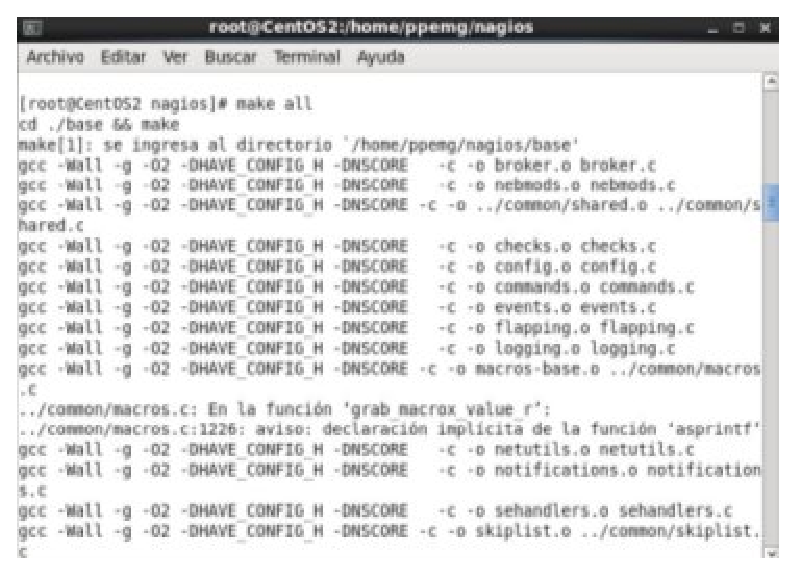
\includegraphics[scale=0.6]{imagenes/opcional2-1.eps}
\caption{Make install.}
\end{center}
\end{figure}

La imagen siguiente muestra la lista de comandos necesaria para continuar con la instalacion de NAGIOS.

\begin{figure}[H]
\begin{center}
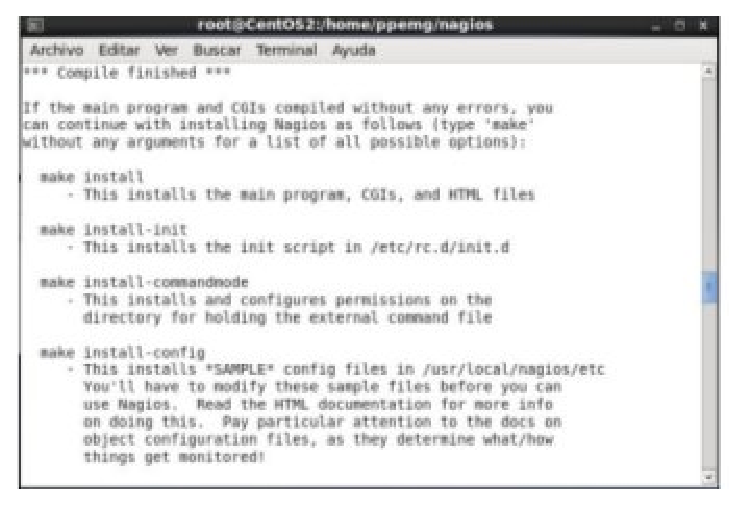
\includegraphics[scale=0.6]{imagenes/opcional2-2.eps}
\caption{Lista de comando que debemos introducir.}
\end{center}
\end{figure}
Ahora cambiamos el correo en el archivo /usr/local/nagios/etc/objects/contacts.cfg

\begin{figure}[H]
\begin{center}
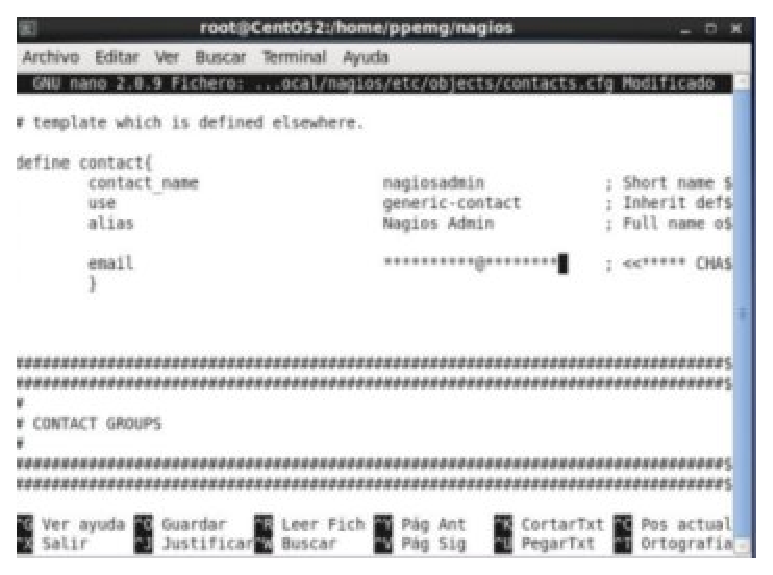
\includegraphics[scale=0.6]{imagenes/opcional2-3.eps}
\caption{Cambio de correo.}
\end{center}
\end{figure}


A continuación ejecutamos la instalación de la interfaz web, creamos el usuario administrados de nagios (nagiosadmin) y reiniciamos apache.

Al ejecutar " make install -webconf " estamos instalando el archivo de configuranción de Nagios / Apache.

\begin{figure}[H]
\begin{center}
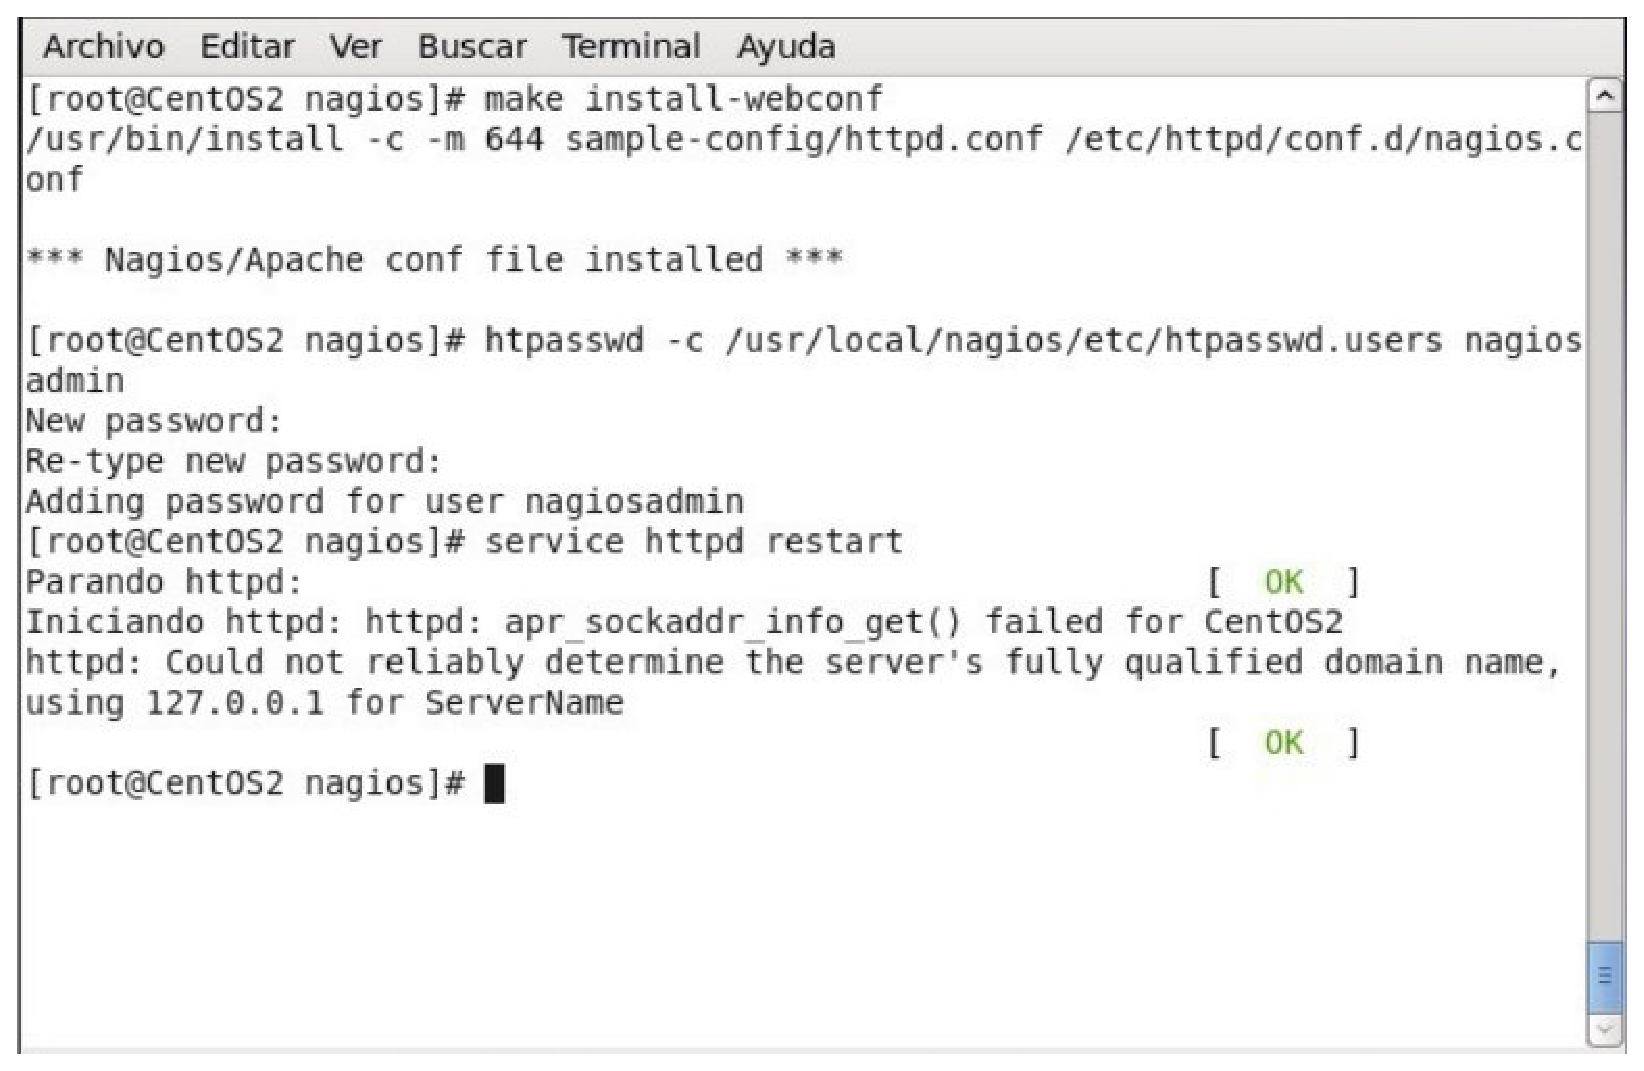
\includegraphics[scale=0.4]{imagenes/opcional2-4.eps}
\caption{Configuración de Nagios con Apache.}
\end{center}
\end{figure}

Ahora repetimos el proceso de instalción con los plugins (extraemos , compilamos e instalamos), solo que esta vez la instacion se realiza con un solo comando "make install". Tras esto, activamos el servicio nagios.

\begin{figure}[H]
\begin{center}
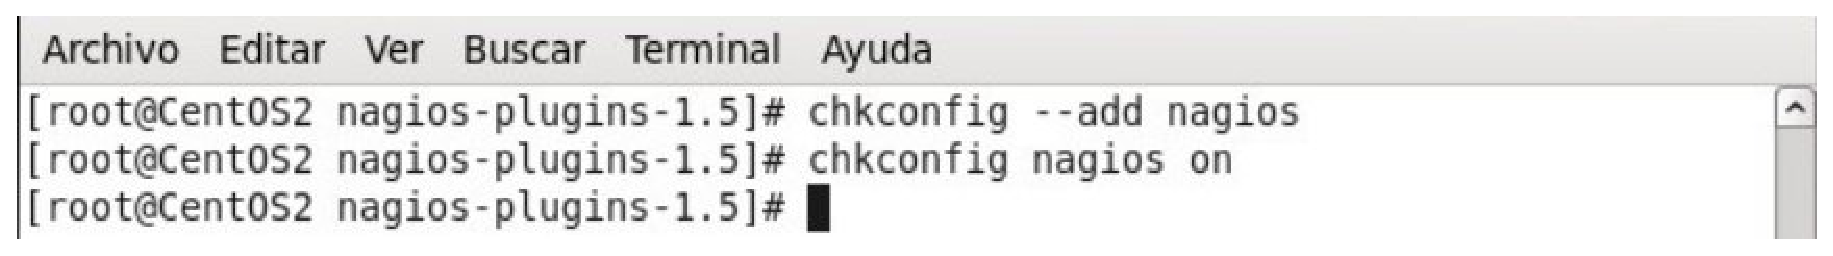
\includegraphics[scale=0.4]{imagenes/opcional2-5.eps}
\caption{Activación de Nagios.}
\end{center}
\end{figure}

Por último nos queda verificar los ficheros de configuración. Para ello usaremos /url/local/nagios/bin/nagios -v /usr/local/nagios/etc/nagios.cfg

\begin{figure}[H]
\begin{center}
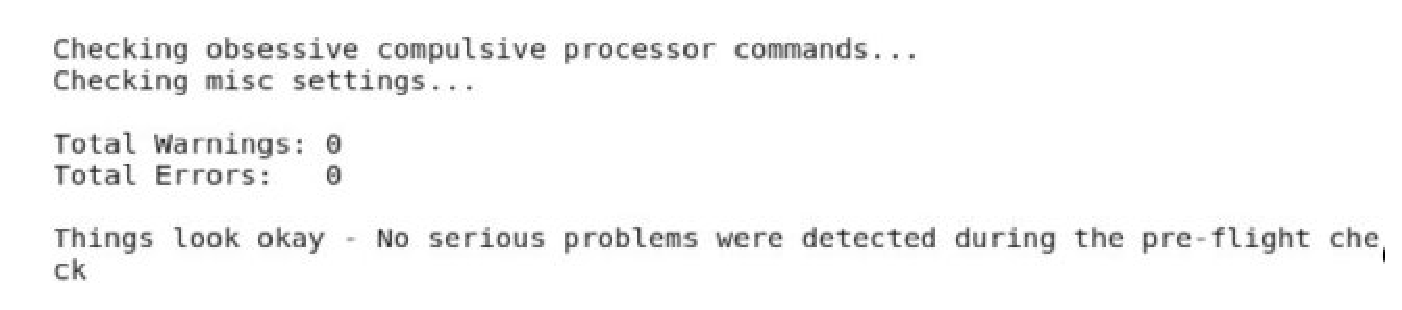
\includegraphics[scale=0.4]{imagenes/opcional2-6.eps}
\caption{Comprobacion de errores en la instalación de Nagios.}
\end{center}
\end{figure}

Como no se ha producido ningún error, iniciamos nagios y accdemos con el usuario nagiosadmin (creado anteriormente) a la direccion /localhost/nagios

\begin{figure}[H]
\begin{center}
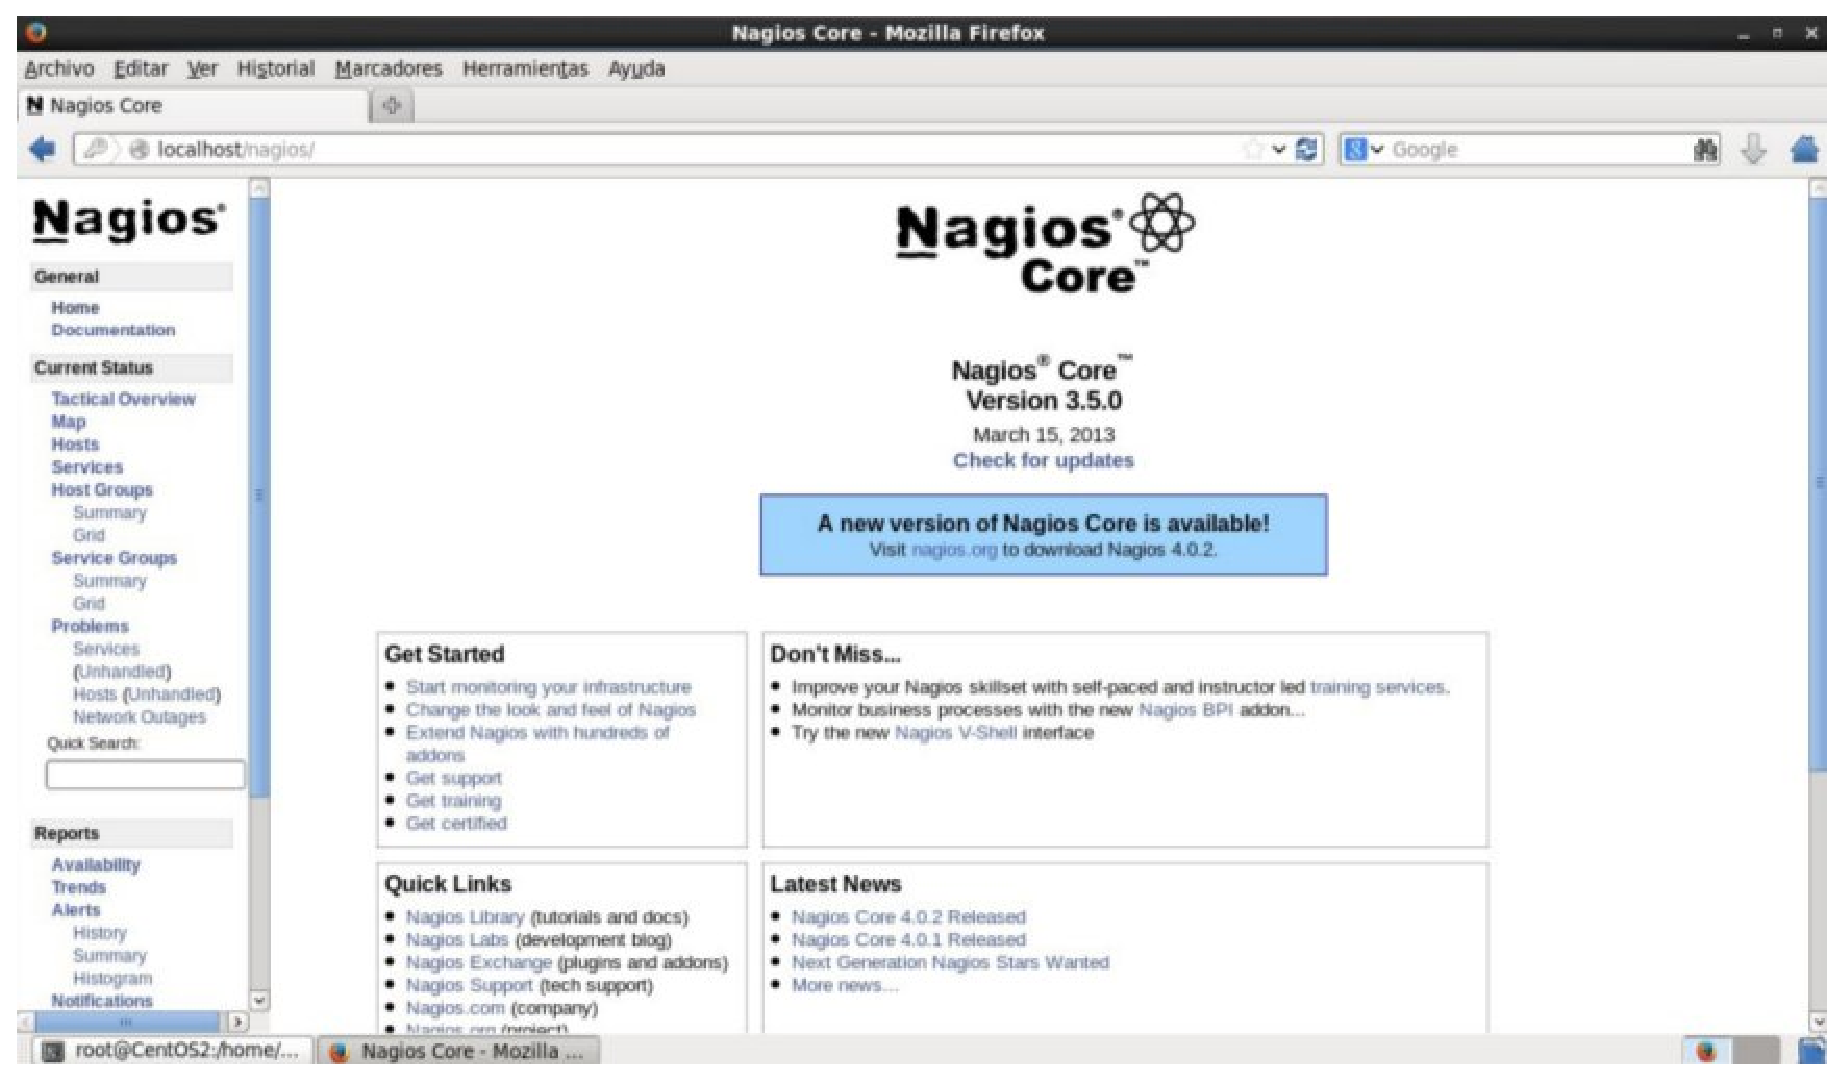
\includegraphics[scale=0.4]{imagenes/opcional2-7.eps}
\caption{Página principal de Nagios.}
\end{center}
\end{figure}

Podemos comprobar los servicios que tenemos activos.

\begin{figure}[H]
\begin{center}
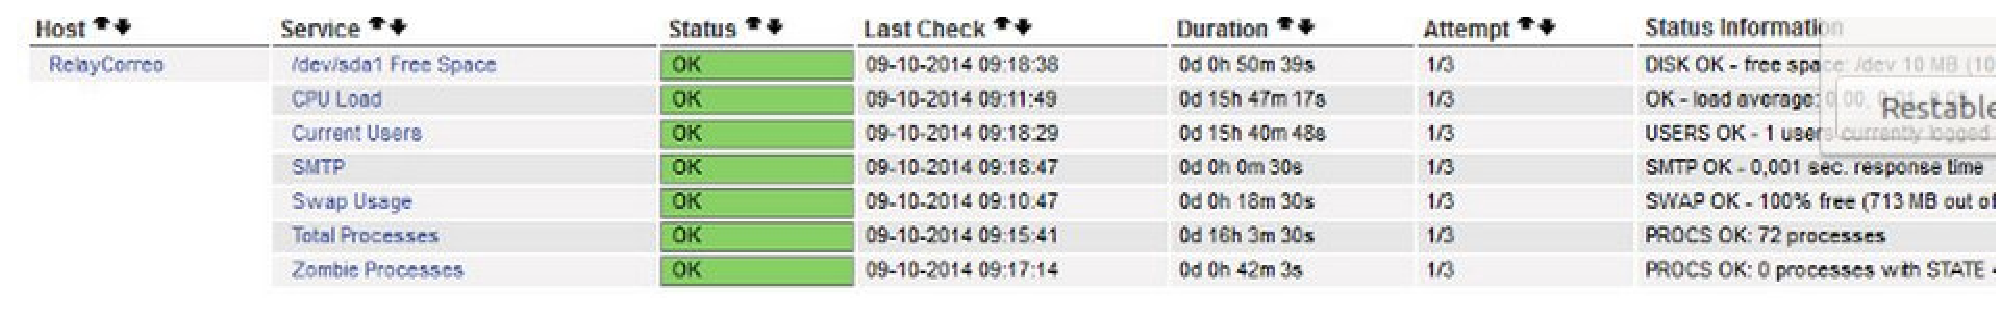
\includegraphics[scale=0.4]{imagenes/opcional2-8.eps}
\caption{Muestra los servicios activos en Nagios.}
\end{center}
\end{figure}

Si alguno de los servicios que se muestran en la figura se mostrase de color rojo y un texto de ¡fail! tendriamos que configurar el archivo de configuracino de nagios y descomentar el apartado donde se activa el servicio por ejemplo en el caso de activar el servicio de monitoreo de correo electronico.

Nagios no es tan simple como las demás aplicaciones que hemos instalado hasta ahora. Para no tener problemas en su instalación se recomienda seguir la guía de instalación oficial de Nagios. \footnote{http://assets.nagios.com/downloads/nagioscore/docs/Installing\_Nagios\_Core\_From\_Source.pdf}

\section*{ Cuestión opcional 5 (CACTI): Pruebe a instalar este monitor en alguno de sus tres sistemas. Realice capturas de pantalla del proceso de instalación y comente capturas de pantalla del programa en ejecución.}


La instalación de CACTI es bastante mas sencilla que la de NAGIOS.


Las referencias usadas han sido las de una página que encontre en google. \footnote{http://www.ubuntugeek.com/how-to-install-cacti-monitoring-tool-in-ubuntu-13-10-server.html}

Para instalar CACTI en ubuntu debemos instroducir el el terminal:
sudo apt-get install cacti-spine


Este comando inicia la instalación de la aplicación.
Como por ejemplo la eleccion de un servidor, que en nuestro caso sera apache, o la configuración de la base de datos.

\begin{figure}[H]
\begin{center}
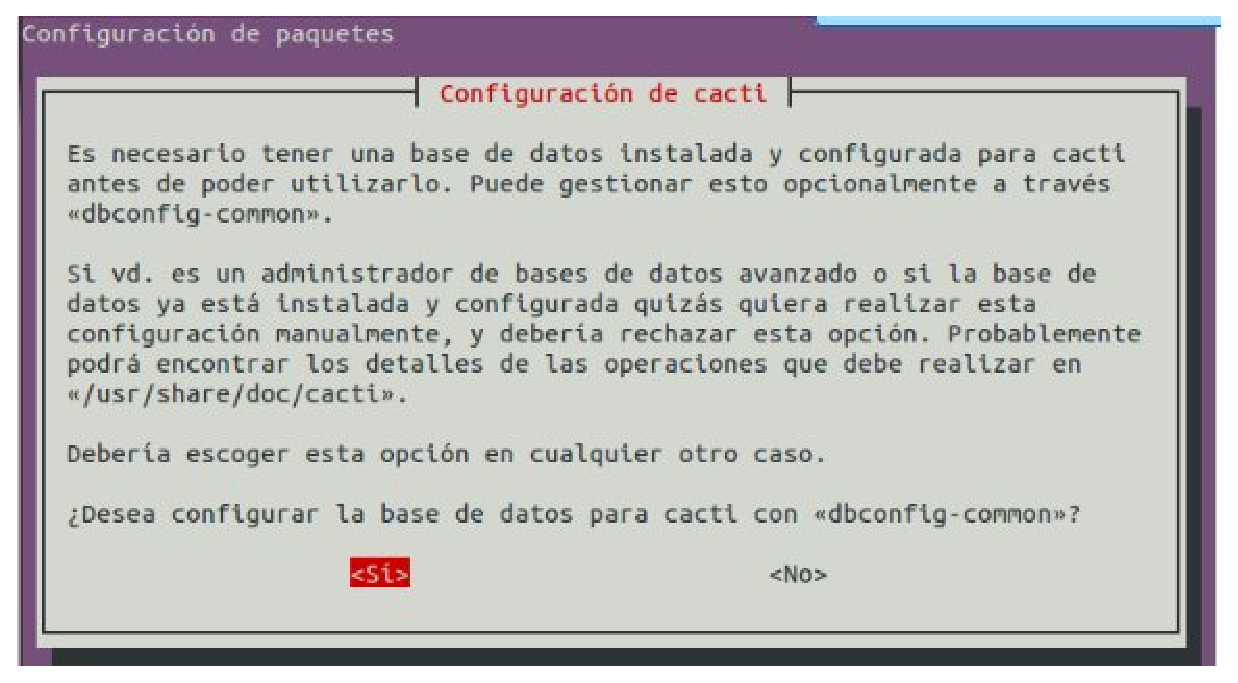
\includegraphics[scale=0.5]{imagenes/opcional5-1.eps}
\caption{Configuración de la base de datos.}
\end{center}
\end{figure}

En la imagen anterior se nos pide configurar la base de datos con CACTI, y la siguiente imagen muestra el proceso de configuración de apache una vez aceptada la pertición de configuración.

\begin{figure}[H]
\begin{center}
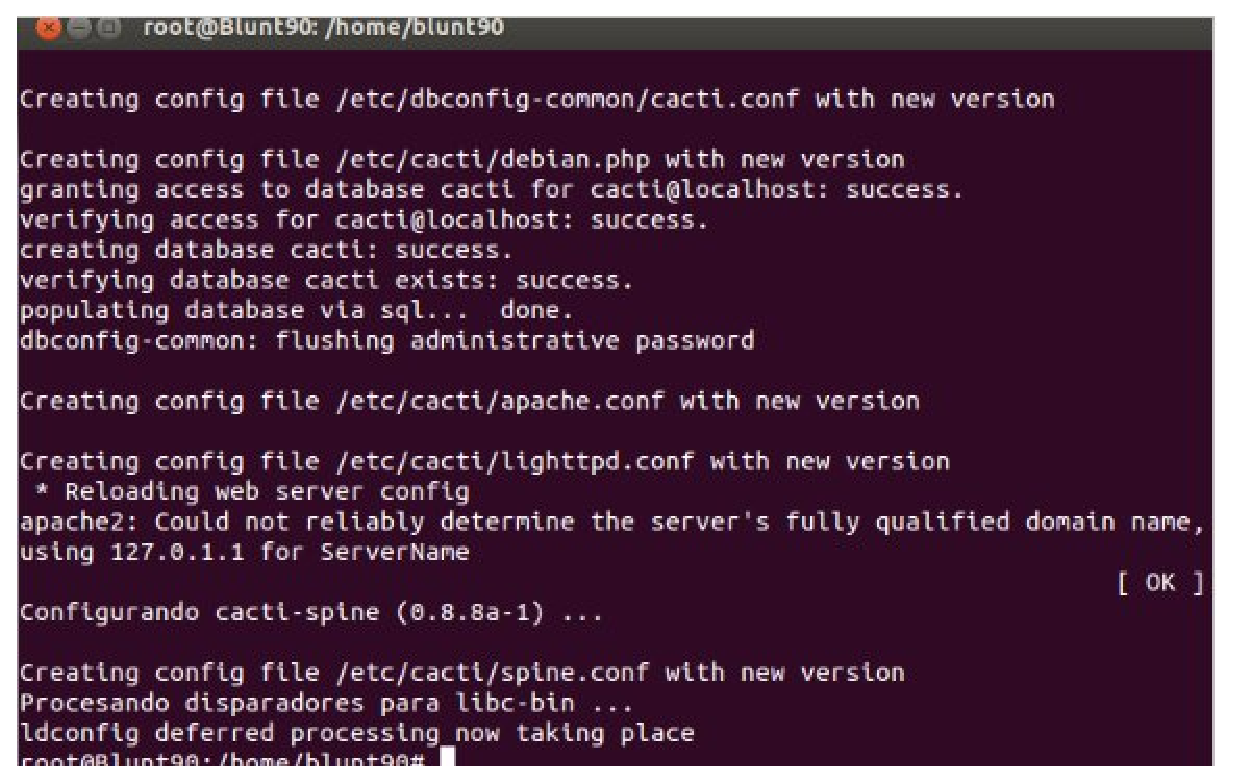
\includegraphics[scale=0.5]{imagenes/opcional5-2.eps}
\caption{Proceso de configuracion de apache para CACTI.}
\end{center}
\end{figure}

La configuracion e instalacion prosiguen introduciendo el usuario adiministrador de la base de datos, creando uno para CACTI y su contraseña, ...

Una vez hecho esto podemos introducir en nuestro navegador http://localhost/cacti/install/ 

Esto nos mostrará una página como la que se muestra a continuación.

\begin{figure}[H]
\begin{center}

\includegraphics[scale=0.5]{imagenes/opcional5-3.eps}
\caption{Inicio guia de instalación CACTI.}
\end{center}
\end{figure}

Pinchamos en next.

La pagina que se nos abrirá a continuacino nos pedira que indiquemos el tipo de instalación que en nuestro caso es "new install", y pinchamos next, que nos volverá a mostrar una pagina que esta vez nos indica si tenemos todos los requisistos necesarios para seguir instalando CACTI.

Una vez hecho esto se nos muestra una pantalla donde logearnos pero tenemos que meter "admin" y "admin" , esto nos volvera a mostrar una pagina igual, como la de la imagen siguiente, pero que esta vez será para cambiar la contraseña.


\begin{figure}[H]
\begin{center}
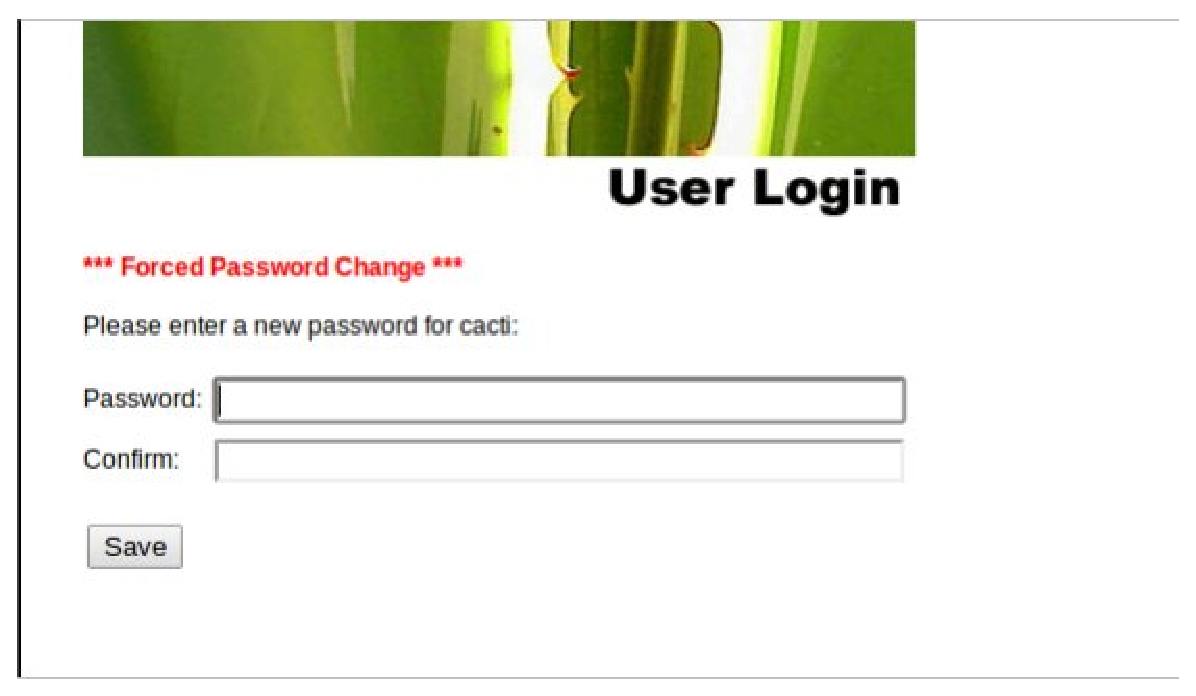
\includegraphics[scale=0.4]{imagenes/opcional5-4.eps}
\caption{Pagina de cambio de contraseña de CACTI.}
\end{center}
\end{figure}


Ahora ya estamos dentro de CACTI logeados como usuarios de CACTI.


\begin{figure}[H]
\begin{center}
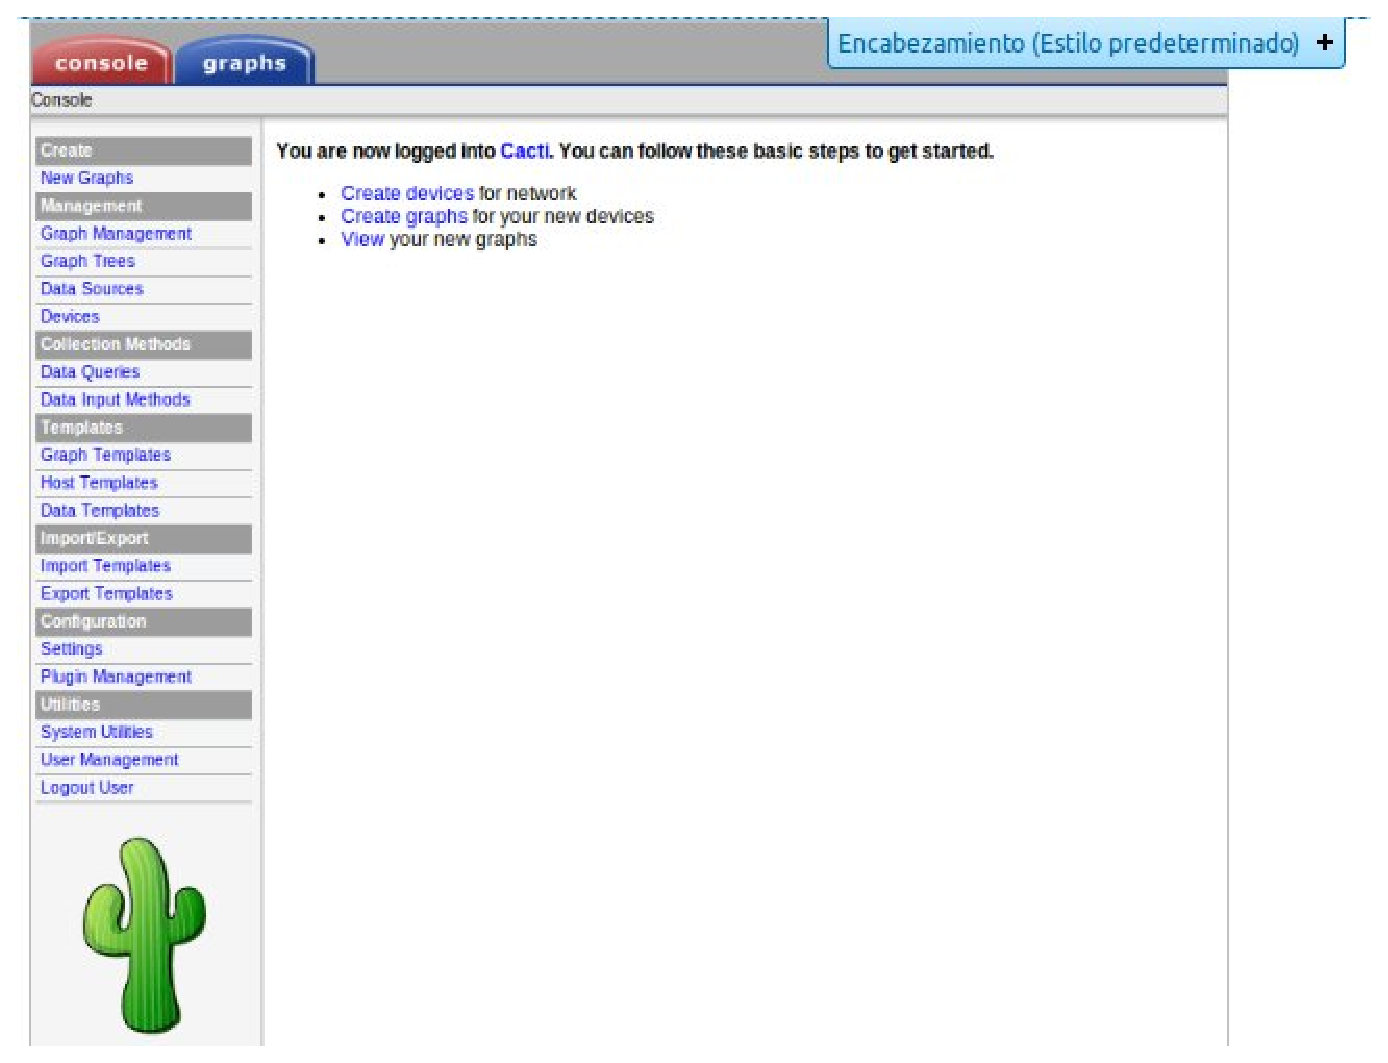
\includegraphics[scale=0.4]{imagenes/opcional5-5.eps}
\caption{Inicio CACTI.}
\end{center}
\end{figure}

Uno de los usos que he probado de CACTI ha sido crear mi propio grafico para controlar el espacio de uno de mis discos, que muestra como resultado la imagen siguiete.

\begin{figure}[H]
\begin{center}
\includegraphics[scale=0.2]{imagenes/opcional5-7.eps}
\caption{Grafico del uso del espacio del disco /dev/sda2.}
\end{center}
\end{figure}

Por ultimo podemos ver todos los graficos que tenemos disponibles, si pinchamos en la pestaña azul de la zona superior de la pantalla. En este apartado de la aplicacion es donde es posible crear tus propios graficos donde elegir que quieres monitorizar.

\begin{figure}[H]
\begin{center}
\includegraphics[scale=0.2]{imagenes/opcional5-8.eps}
\caption{Página CACTI para la creación y elección de gráficos.}
\end{center}
\end{figure}

Al igual que en el caso de Nagios, aunque esta aplicación es mucho mas sencilla, hay muchos tutoriales en internet de como hacerlo, pero se recomienda encarecidamente que si desea instalar este sistema consulte la guía de instalación oficial de CACTI \footnote{http://www.cacti.net/downloads/docs/html/install\_unix.html} y la de configuración \footnote{http://www.cacti.net/downloads/docs/html/unix\_configure\_cacti.html}

\end{document}